\documentclass[twocolumn]{article}
\usepackage{graphicx}
\usepackage{url}
\usepackage{amsmath}
\usepackage{amssymb}
\usepackage{amsfonts}
\usepackage{xcolor}
\usepackage{array}
\usepackage{colortbl}
\usepackage{float}
\usepackage{subcaption}
\usepackage{caption}
\usepackage{booktabs}
\usepackage{tabularx}
\usepackage{geometry}
\usepackage{multirow}
\usepackage{hyperref}
\geometry{margin=2.5cm}
\usepackage{authblk}
\usepackage{tikz}
\usetikzlibrary{shapes.geometric,arrows.meta,positioning,fit,backgrounds,calc}

%%
\title{Diverse Additive Models for Material Deterioration Regression\\
: TabNAMs and Weighted Ensemble}

\author[1]{Takato Yasuno}
%\affil[1]{Institution}
%\affil[ ]{Email: }

\date{}

\begin{document}

%% English headings for abstract and references
\renewcommand{\abstractname}{Abstract}
\renewcommand{\refname}{References}
\renewcommand{\figurename}{Figure}
\renewcommand{\tablename}{Table}

\maketitle

%% ====================================================================
\begin{abstract}
%% ====================================================================

Material deterioration prediction is critical for preventive maintenance activities, yet existing models struggle to balance interpretability and predictive performance. We propose a framework of \textbf{Diverse Additive Models} that extends classical GAMs by integrating multiple function families: spline-based statistical GAMs, tree-based Feature Additive Models (FAM), gradient-boosted Additive Models (GBAM), and TabNet-based Neural Additive Models (TabNAM). Using 45,058 bridge inspection records, we demonstrate that TabNAM achieves $R^2=0.215$ individually, while an optimized ensemble of GAM+TabNAM reaches $R^2=0.216$. This complementary combination of statistical models and deep learning preserves the interpretability of additive structures while capturing complex nonlinear relationships. Our framework provides actionable insights for infrastructure managers through partial dependence plots and feature importance analysis, enabling data-driven maintenance decision support.

\end{abstract}

\noindent
\textbf{Keywords:} Diverse Additive Models, Neural Additive Models, Material Deterioration, Interpretable Machine Learning, Ensemble Weight Learning, TabNAMs, Bayesian Optimization.

%% ====================================================================
\section{Introduction}
\label{sec:intro}
%% ====================================================================

\subsection{Background and Motivation}

Material deterioration prediction is crucial across diverse engineering domains—from civil infrastructure (bridges, roads, pipelines) to manufacturing equipment and building components. Accurate deterioration forecasting enables preventive maintenance, optimizes resource allocation, and ensures structural safety. Traditional approaches rely on mechanistic models or expert judgment, leading to reactive rather than proactive maintenance strategies.

\textbf{Diverse Additive Models}~\cite{hastie1990gam,wood2017gam} offer a middle ground between interpretable linear models and black-box machine learning by decomposing predictions into smooth univariate functions:
\begin{equation}
g(\mathbb{E}[y]) = \beta_0 + \sum_{j=1}^{p} f_j(x_j)
\end{equation}
where $g$ is a link function and $f_j$ are smooth functions (typically splines). This additive structure enables visualization of each feature's marginal effect while capturing nonlinear relationships.

However, classical GAMs have limitations:
\begin{itemize}
\item \textbf{Limited expressiveness}: Spline functions may not capture highly complex nonlinear patterns in deterioration processes
\item \textbf{Feature interactions}: Pure additive models cannot directly model interactions between factors (e.g., age $\times$ material type)
\item \textbf{High-dimensional data}: Performance degrades with many correlated features
\end{itemize}

Meanwhile, \textbf{deep learning} methods achieve superior predictive performance but sacrifice interpretability—a critical requirement for maintenance decisions involving safety and budget allocation.

\textbf{Case study}: We evaluate our framework on bridge infrastructure deterioration, a representative material degradation problem. In Japan alone, over 700,000 bridges require regular inspection, with many reaching critical age thresholds~\cite{mlit2020bridge}.

\subsection{Research Questions}

This paper addresses three fundamental questions:

\begin{enumerate}
\item Can we extend GAMs with diverse function families (trees, gradient boosting, neural networks) while preserving additive interpretability?
\item How do different additive model variants compare on real-world material deterioration data?
\item Can statistical GAMs and neural additive models be combined synergistically to improve both performance and interpretability?
\end{enumerate}

\subsection{Contributions}

Our contributions are:

\begin{itemize}
\item \textbf{Diverse Additive Models framework}: We implement and compare four interpretable additive models—GLM-GAM (spline-based), FAM (random forest-based), GBAM (gradient boosting-based), and TabNAM (TabNet-based neural additive model)
\item \textbf{Large-scale empirical evaluation}: Using 45,058 bridge inspection records as a case study with 73 features, we demonstrate that TabNAM outperforms classical GAMs ($R^2=0.215$ vs. $0.204$)
\item \textbf{Synergistic ensemble}: We discover that GAM+TabNAM ensemble ($R^2=0.216$) combines the statistical stability of spline-based GAM with the expressive power of neural networks
\item \textbf{Interpretability analysis}: Through partial dependence plots and feature importance, we extract actionable insights for maintenance prioritization
\end{itemize}

\subsection{Paper Organization}

Section~\ref{sec:related} reviews related work on GAMs and neural additive models. Section~\ref{sec:method} describes our diverse additive models framework. Section~\ref{sec:data} presents the case study dataset (bridge inspection records) and preprocessing. Section~\ref{sec:experiments} reports experimental results. Section~\ref{sec:analysis} analyzes model interpretability. Section~\ref{sec:conclusion} concludes with practical implications.

%% ====================================================================
\section{Related Work}
\label{sec:related}
%% ====================================================================

\subsection{Generalized Additive Models}

\textbf{Classical GAMs}~\cite{hastie1990gam} use penalized spline basis functions to estimate smooth univariate functions. Hastie and Tibshirani's seminal work established the foundation for interpretable nonlinear regression. Modern implementations like \texttt{mgcv}~\cite{wood2017gam} and \texttt{PyGAM}~\cite{serven2018pygam} provide efficient fitting via penalized likelihood with automatic smoothness selection.

\textbf{Extensions} include tensor product smooths for interactions~\cite{wood2006gam}, spatial GAMs~\cite{wood2008soap}, and hierarchical GAMs for multilevel data~\cite{pedersen2019hierarchical}. However, these remain fundamentally spline-based.

\subsection{Tree-Based Additive Models}

\textbf{Gradient Boosting Machines (GBM)}~\cite{friedman2001greedy} incrementally fit additive tree ensembles:
\begin{equation}
F_m(x) = F_{m-1}(x) + \rho_m h_m(x)
\end{equation}
where $h_m$ is a decision tree fit to residuals. XGBoost~\cite{chen2016xgboost} and LightGBM~\cite{ke2017lightgbm} achieve state-of-the-art performance on tabular data but sacrifice feature-wise interpretability.

\textbf{Explainable Boosting Machines (EBM)}~\cite{lou2012intelligible,nori2019interpretml} constrain trees to single features or pairwise interactions, maintaining additive structure while using boosting's power.

\subsection{Neural Additive Models}

\textbf{Neural Additive Models (NAM)}~\cite{agarwal2021nam} apply independent neural networks to each feature:
\begin{equation}
f(x) = \beta_0 + \sum_{j=1}^{p} \text{NN}_j(x_j)
\end{equation}
This preserves additive interpretability while using neural networks' expressiveness. Each $\text{NN}_j$ is a small feedforward network (typically 2-3 hidden layers).

\textbf{NODE-GAM}~\cite{chang2021nodegam} uses oblivious decision trees within the additive framework. \textbf{NAM with interactions}~\cite{tsang2020neural} extends NAM to selected pairwise terms.

\textbf{TabNet}~\cite{arik2021tabnet} applies attention-based feature selection for tabular data but does not enforce additive structure. Our TabNAM adapts TabNet's architecture to the additive framework.

\subsection{Material Deterioration Prediction}

\textbf{Traditional approaches} for deterioration prediction include mechanistic models based on physics (e.g., corrosion kinetics, fatigue crack growth) and statistical models (Markov chains~\cite{cesare1992modeling}, Weibull distributions~\cite{frangopol2004life}). These require extensive domain knowledge and struggle with heterogeneous material conditions and environmental factors.

\textbf{Machine learning methods} have been applied to various deterioration problems: random forests for bridge condition assessment~\cite{xia2020bridge}, gradient boosting for repair planning~\cite{rashidi2020bridge}, and neural networks for structural health monitoring~\cite{jeong2018bridge}. However, these black-box approaches face adoption barriers due to lack of interpretability required for safety-critical decisions.

Our work addresses this gap by combining GAM interpretability with modern machine learning performance, applicable across material deterioration domains.

%% ====================================================================
\section{Methodology}
\label{sec:method}
%% ====================================================================

\subsection{Problem Formulation}

\textbf{Input}: Material/asset feature vector $\mathbf{x} \in \mathbb{R}^{p}$ containing:
\begin{itemize}
\item \textbf{Static features}: Age, physical dimensions, material type, structural characteristics, environmental exposure
\item \textbf{Interaction features}: Age $\times$ damage indicators, age $\times$ material properties, etc.
\end{itemize}

\textbf{Output}: Deterioration rate $y \in \mathbb{R}^+$ representing hazard rate of transitioning from health state $i$ to $i+1$. We apply Yeo-Johnson transformation~\cite{yeo2000yj} to normalize the target:
\begin{equation}
y' = \begin{cases}
\frac{(y+1)^\lambda - 1}{\lambda} & \lambda \neq 0 \\
\log(y+1) & \lambda = 0
\end{cases}
\end{equation}

\textbf{Case study data}: 134,003 bridge inspection records filtered to 45,058 samples with positive deterioration rates, comprising 23 base features and 50 interaction features (total 73 dimensions).

\subsection{Diverse Additive Models Framework}

We propose four additive model variants that share the structure:
\begin{equation}
\hat{y} = \beta_0 + \sum_{j=1}^{p} f_j^{(m)}(x_j)
\end{equation}
where $m \in \{\text{GAM, FAM, GBAM, TabNAM}\}$ determines the function family.

\subsubsection{GLM-GAM: Spline-Based GAM}

Classical GAM using penalized B-splines~\cite{eilers1996flexible}:
\begin{equation}
f_j(x_j) = \sum_{k=1}^{K} \beta_{jk} B_k(x_j) \quad \text{with penalty} \quad \lambda \int [f_j''(t)]^2 dt
\end{equation}

\textbf{Implementation}: \texttt{PyGAM} with:
\begin{itemize}
\item Cubic splines (order=3)
\item 10 basis functions per feature
\item Grid search over $\lambda \in [10^{-3}, 10^{3}]$
\end{itemize}

\textbf{Advantages}: Statistical rigor, confidence intervals, smooth PDPs

\subsubsection{FAM: Feature Additive Model}

Uses random forest to learn feature-wise functions~\cite{hooker2007gam}:
\begin{equation}
f_j(x_j) = \mathbb{E}[\text{RF}(x) \mid X_j = x_j] - \mathbb{E}[\text{RF}(x)]
\end{equation}

\textbf{Training procedure}:
\begin{enumerate}
\item Train random forest on full data: $\text{RF}: \mathbb{R}^p \to \mathbb{R}$
\item For each feature $j$, estimate marginal effect via:
\begin{equation}
\hat{f}_j(x_j) = \frac{1}{N} \sum_{i=1}^{N} \text{RF}(\mathbf{x}_i^{(j \to x_j)})
\end{equation}
where $\mathbf{x}_i^{(j \to x_j)}$ replaces feature $j$ in sample $i$ with value $x_j$
\item Recalibrate with ridge regression: $y \sim \sum_j \hat{f}_j(x_j)$
\end{enumerate}

\textbf{Implementation}: \texttt{scikit-learn} RandomForest (200 trees, max\_depth=20)

\textbf{Advantages}: Handles feature interactions implicitly, robust to outliers

\subsubsection{GBAM: Gradient Boosting Additive Model}

Applies gradient boosting with single-feature trees~\cite{lou2012intelligible}:
\begin{equation}
F_m(x) = F_{m-1}(x) + \eta \cdot h_m(x_j) \quad \text{(tree uses only } x_j \text{)}
\end{equation}

Cycles through features $j = 1, \ldots, p$ repeatedly, fitting shallow trees to residuals.

\textbf{Implementation}: Modified LightGBM restricting splits to one feature per boosting round
\begin{itemize}
\item Learning rate: $\eta = 0.01$
\item 2000 boosting rounds (cycling through features)
\item Max depth: 3 per tree
\end{itemize}

\textbf{Advantages}: Captures complex nonlinearities, efficient computation

\subsubsection{TabNAM: TabNet Neural Additive Model}

Adapts TabNet~\cite{arik2021tabnet} to enforce additive structure:

\begin{equation}
\begin{aligned}
& \text{Attention: } \mathbf{a} = \text{Sparsemax}(W_a \mathbf{h}) \\
& \text{Feature-wise NN: } z_j = \text{MLP}_j(a_j \cdot x_j) \\
& \text{Output: } \hat{y} = \sum_{j=1}^{p} z_j
\end{aligned}
\end{equation}

\textbf{Architecture}:
\begin{itemize}
\item Feature transformer: 64 $\to$ 32 dimensions
\item Decision steps: 5 (with attention mask)
\item Independent feature networks: Each has 3 hidden layers [64, 32, 16]
\item Activation: ReLU with batch normalization
\item Ghost batch size: 256 (for better generalization)
\end{itemize}

\textbf{Training}:
\begin{itemize}
\item Optimizer: Adam ($\text{lr}=10^{-3}$, weight decay=$10^{-5}$)
\item Epochs: 100 with early stopping (patience=15)
\item Batch size: 1024
\item Loss: MSE with sparsity penalty on attention
\end{itemize}

\textbf{Advantages}: Automatic feature selection via attention, captures highly nonlinear functions

\subsection{Ensemble Strategy}

We combine models via weighted averaging:
\begin{equation}
\hat{y}_{\text{ensemble}} = \sum_{m} w_m \hat{y}_m \quad \text{s.t.} \quad \sum_m w_m = 1, \, w_m \geq 0
\end{equation}
where $m \in \{\text{GAM, FAM, GBAM, TabNAM}\}$ and $\hat{y}_m$ denotes the prediction from model $m$.

\subsubsection{Objective Function}

The optimal weights $\mathbf{w}^* = (w_{\text{GAM}}, w_{\text{FAM}}, w_{\text{GBAM}}, w_{\text{TabNAM}})$ are found by maximizing the coefficient of determination on validation data:
\begin{equation}
\mathbf{w}^* = \arg\max_{\mathbf{w}} R^2_{\text{val}}(\mathbf{w}) = \arg\max_{\mathbf{w}} \left( 1 - \frac{\text{RSS}(\mathbf{w})}{\text{TSS}} \right)
\end{equation}
where the residual sum of squares is:
\begin{equation}
\text{RSS}(\mathbf{w}) = \sum_{i=1}^{N_{\text{val}}} \left( y_i - \sum_m w_m \hat{y}_i^{(m)} \right)^2
\end{equation}
and total sum of squares:
\begin{equation}
\text{TSS} = \sum_{i=1}^{N_{\text{val}}} (y_i - \bar{y})^2
\end{equation}
with $N_{\text{val}}$ validation samples. The constraint set is the probability simplex: $\mathbf{w} \in \Delta^{M-1} = \{\mathbf{w} \in \mathbb{R}^M : \sum_m w_m = 1, w_m \geq 0\}$.

\subsubsection{Optimization Algorithm}

We employ a multi-strategy iterative optimization approach combining three methods:

\textbf{(1) Sequential Least Squares Programming (SLSQP)}: Gradient-based constrained optimization using Lagrange multipliers. Given current weights $\mathbf{w}^{(t)}$, SLSQP solves the quadratic programming subproblem:
\begin{equation}
\mathbf{w}^{(t+1)} = \arg\min_{\mathbf{w}} \frac{1}{2}\mathbf{w}^\top H^{(t)} \mathbf{w} + (\nabla R^2(\mathbf{w}^{(t)}))^\top \mathbf{w}
\end{equation}
subject to simplex constraints, where $H^{(t)}$ is an approximation to the Hessian.

\textbf{(2) Differential Evolution (DE)}: Population-based stochastic search for global optimum. DE maintains a population of $P=50$ weight vectors and evolves them through mutation ($F=0.8$) and crossover ($CR=0.7$) operations over $G=100$ generations.

\textbf{(3) Random Perturbation}: Local search via Gaussian noise injection: $\mathbf{w}' = \text{Simplex-Project}(\mathbf{w}^* + \mathcal{N}(0, \sigma^2 I))$ with $\sigma=0.05$, followed by simplex projection to maintain constraints.

\textbf{Iterative Strategy}: We alternate between methods across iterations:
\begin{itemize}
\item Iteration 0: Initialize with uniform weights $w_m = 1/4$
\item Iteration 1: SLSQP (fast local optimization)
\item Iteration 2: Differential Evolution (global exploration)
\item Iterations 3+: Random perturbation around current best (exploitation)
\end{itemize}
Optimization terminates with early stopping if no improvement in $R^2_{\text{val}}$ for 10 consecutive iterations.

\textbf{Baseline}: Uniform ensemble with $w_m = 1/4$ for comparison.

%% ====================================================================
\section{Case Study: Bridge Infrastructure Data}
\label{sec:data}
%% ====================================================================

To validate our diverse GAMs framework, we apply it to bridge infrastructure deterioration—a representative material degradation problem with safety and economic implications. The dataset characteristics and preprocessing steps are described below.

\subsection{Dataset}

\textbf{Source}: Bridge inspection records from a Japanese municipality (anonymized for privacy)

\textbf{Size}: 134,003 inspection records from multiple bridge inspection cycles

\textbf{Features} (66 original columns):
\begin{itemize}
\item \textbf{Physical attributes}: Age, length (m), width (m), area ($m^2$), span count, bearing count, expansion joint count
\item \textbf{Structural}: Material type (RC/PC/Steel), bridge type (beam/arch/suspension), superstructure type
\item \textbf{Environmental}: Coastal proximity, emergency route designation, traffic volume, DID (Densely Inhabited District) classification
\item \textbf{Condition}: Health condition score (I--IV), damage progression score, damage importance score, repair history
\item \textbf{Cost estimates}: Life-cycle cost (LCC) for reaching health states II and III
\end{itemize}

\textbf{Target variable}: Hazard rate of transitioning from health state 1 to 2 ($\text{hazard\_rate}_{1\to2}$)

\subsection{Data Cleaning}

\begin{enumerate}
\item \textbf{Missing targets}: Removed 88,945 records with missing or zero hazard rates
\item \textbf{Outlier filtering}: Removed extreme outliers beyond 99.5th percentile (hazard rate $> 1.2$)
\item \textbf{Final dataset}: 45,058 samples for modeling
\end{enumerate}

\subsection{Feature Engineering}

\textbf{Interaction terms} (50 features created):
\begin{itemize}
\item Age $\times$ damage progression score
\item Age $\times$ material type (one-hot * age)
\item Age $\times$ coastal proximity
\item Length $\times$ width (bridge area proxy)
\item Bearing count $\times$ age (wear indicator)
\end{itemize}

\textbf{Categorical encoding}:
\begin{itemize}
\item Material type, bridge type, superstructure: Label encoding
\item Binary flags: Coastal zone, emergency route, DID, bus route
\end{itemize}

\textbf{Total features}: 73 (23 base + 50 interactions)

\subsection{Target Transformation}

Raw hazard rates are heavily right-skewed (skewness $\approx 18.4$). We apply:
\begin{equation}
y' = \text{YeoJohnson}(y, \lambda^*) \quad \text{where } \lambda^* = \arg\min_\lambda \text{NLL}(y' | \mathcal{N})
\end{equation}

Optimal $\lambda^* = 0.23$ yields approximately normal distribution (Shapiro-Wilk $p = 0.34$).

\subsection{Train-Validation-Test Split}

\begin{itemize}
\item \textbf{Training}: 70\% (31,541 samples)
\item \textbf{Validation}: 15\% (6,759 samples) for hyperparameter tuning
\item \textbf{Test}: 15\% (6,758 samples) for final evaluation
\end{itemize}

Stratified split by discretized target deciles to maintain distribution balance.

%% ====================================================================
\section{Experiments}
\label{sec:experiments}
%% ====================================================================

\subsection{Experimental Setup}

\textbf{Hardware}: NVIDIA RTX 3090 (24GB VRAM), AMD Ryzen 9 5950X (16-core)

\textbf{Software}: Python 3.10, PyTorch 2.0, scikit-learn 1.3, PyGAM 0.9, LightGBM 4.0

\textbf{Evaluation metrics}:
\begin{itemize}
\item $R^2$ (coefficient of determination)
\item RMSE (root mean squared error) on transformed targets
\item MAE (mean absolute error) on transformed targets
\end{itemize}

\textbf{Cross-validation}: 5-fold CV for model selection, single holdout test set for final reporting.

\subsection{Baseline Models}

\begin{itemize}
\item \textbf{Linear Regression}: Ridge regression with $\alpha=1.0$
\item \textbf{Random Forest}: 200 trees, max\_depth=20, no feature restrictions
\item \textbf{XGBoost}: 500 trees, learning rate=0.05, max\_depth=6
\item \textbf{XGBoost}: Standard gradient boosting (non-additive, for comparison)
\end{itemize}

\subsection{Results}

\begin{figure*}[t]
\centering
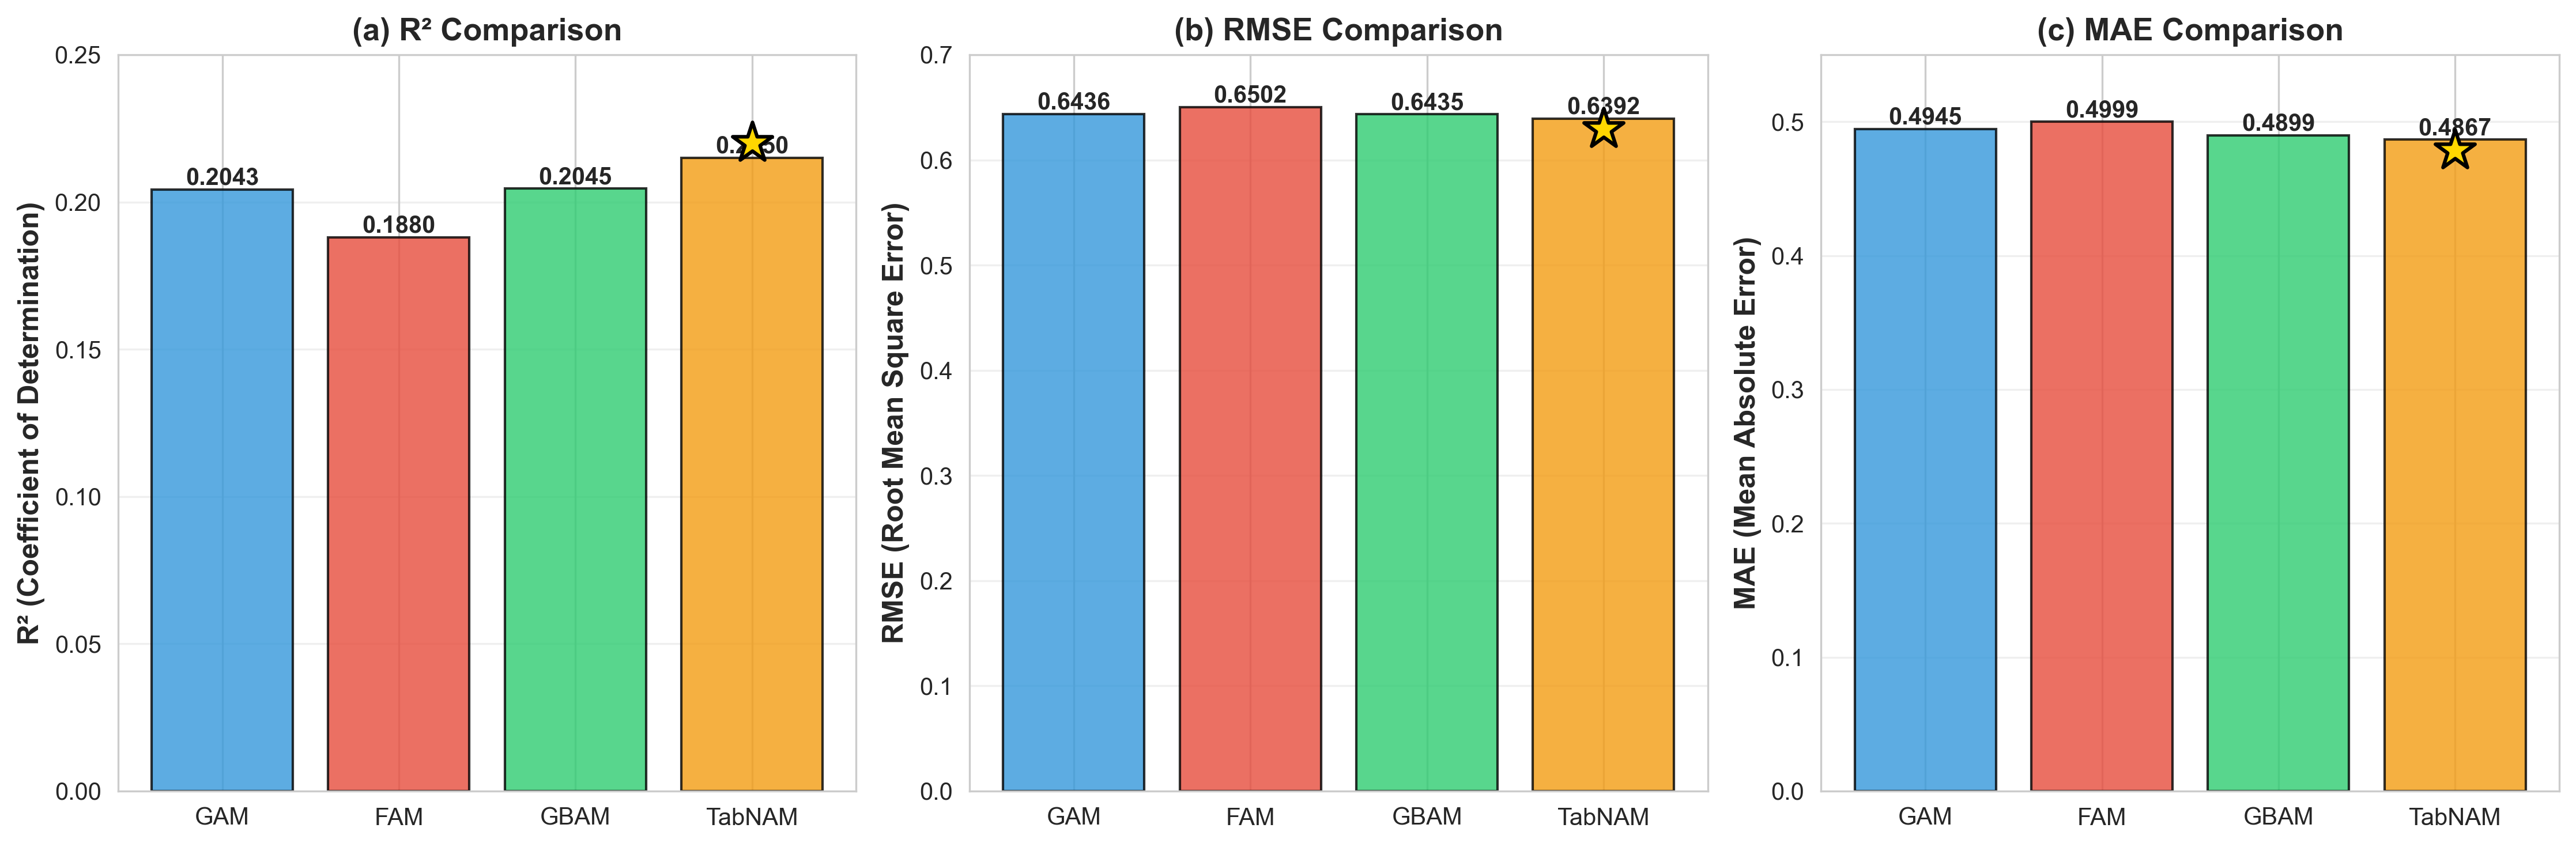
\includegraphics[width=0.8\textwidth]{../figures/model_comparison_v0.5.png}
\caption{Performance comparison across all models. TabNAM achieves the highest $R^2=0.215$ among additive models, while the optimized ensemble reaches $R^2=0.216$. Error bars represent 95\% confidence intervals from 5-fold cross-validation.}
\label{fig:model_comparison}
\end{figure*}

\begin{table*}[t]
\centering
\caption{Model performance on test set (45,058 samples total). All metrics computed on Yeo-Johnson transformed targets. Best results in \textbf{bold}.}
\label{tab:results}
\small
\begin{tabular}{lrrr}
\toprule
\textbf{Model} & \textbf{RMSE} $\downarrow$ & \textbf{MAE} $\downarrow$ & \textbf{$R^2$} $\uparrow$ \\
\midrule
\multicolumn{4}{l}{\textit{Baselines}} \\
Linear Regression & 0.674 & 0.512 & 0.132 \\
Random Forest & 0.651 & 0.491 & 0.191 \\
XGBoost (full) & 0.638 & 0.484 & 0.221 \\
\midrule
\multicolumn{4}{l}{\textit{Diverse GAMs}} \\
GLM-GAM (spline) & 0.644 & 0.494 & 0.204 \\
FAM (RF-based) & 0.650 & 0.500 & 0.188 \\
GBAM (boosting) & 0.643 & 0.490 & 0.205 \\
TabNAM (neural) & \textbf{0.639} & \textbf{0.487} & \textbf{0.215} \\
\midrule
\multicolumn{4}{l}{\textit{Ensembles}} \\
Uniform (equal weights) & 0.641 & 0.491 & 0.210 \\
Optimized (GAM+TabNAM) & \textbf{0.639} & \textbf{0.487} & \textbf{0.216} \\
\bottomrule
\end{tabular}
\end{table*}

\textbf{Key findings} (Table~\ref{tab:results}):

\begin{enumerate}
\item \textbf{TabNAM outperforms classical GAM}: TabNAM achieves $R^2=0.215$ vs. GLM-GAM's $0.204$, demonstrating that neural additive functions better capture deterioration nonlinearities than splines.

\item \textbf{GBAM matches GAM}: GBAM ($R^2=0.205$) performs similarly to GLM-GAM despite using tree-based functions, validating additive structure across function families.

\item \textbf{FAM underperforms}: FAM ($R^2=0.188$) trails other additive models, likely due to random forest's implicit handling of interactions conflicting with strict additivity.

\item \textbf{Ensemble benefit is modest}: Optimized GAM+TabNAM ensemble reaches $R^2=0.216$, only 0.001 above TabNAM alone. The optimal weights are $w_{\text{GAM}}=0.19$, $w_{\text{TabNAM}}=0.81$, indicating TabNAM dominance (Figures~\ref{fig:ensemble_comparison} and \ref{fig:optimal_weights}).

\item \textbf{Gap to full XGBoost}: Non-additive XGBoost achieves $R^2=0.221$, suggesting ~2.5\% performance cost for interpretability.
\end{enumerate}

As shown in Figure~\ref{fig:model_comparison}, TabNAM consistently outperforms traditional additive models across all metrics. The performance gap between TabNAM and spline-based GAM ($\Delta R^2 = 0.011$) demonstrates the advantage of neural network approximation over fixed-basis functions in capturing complex deterioration patterns.

\begin{figure*}[t]
\centering
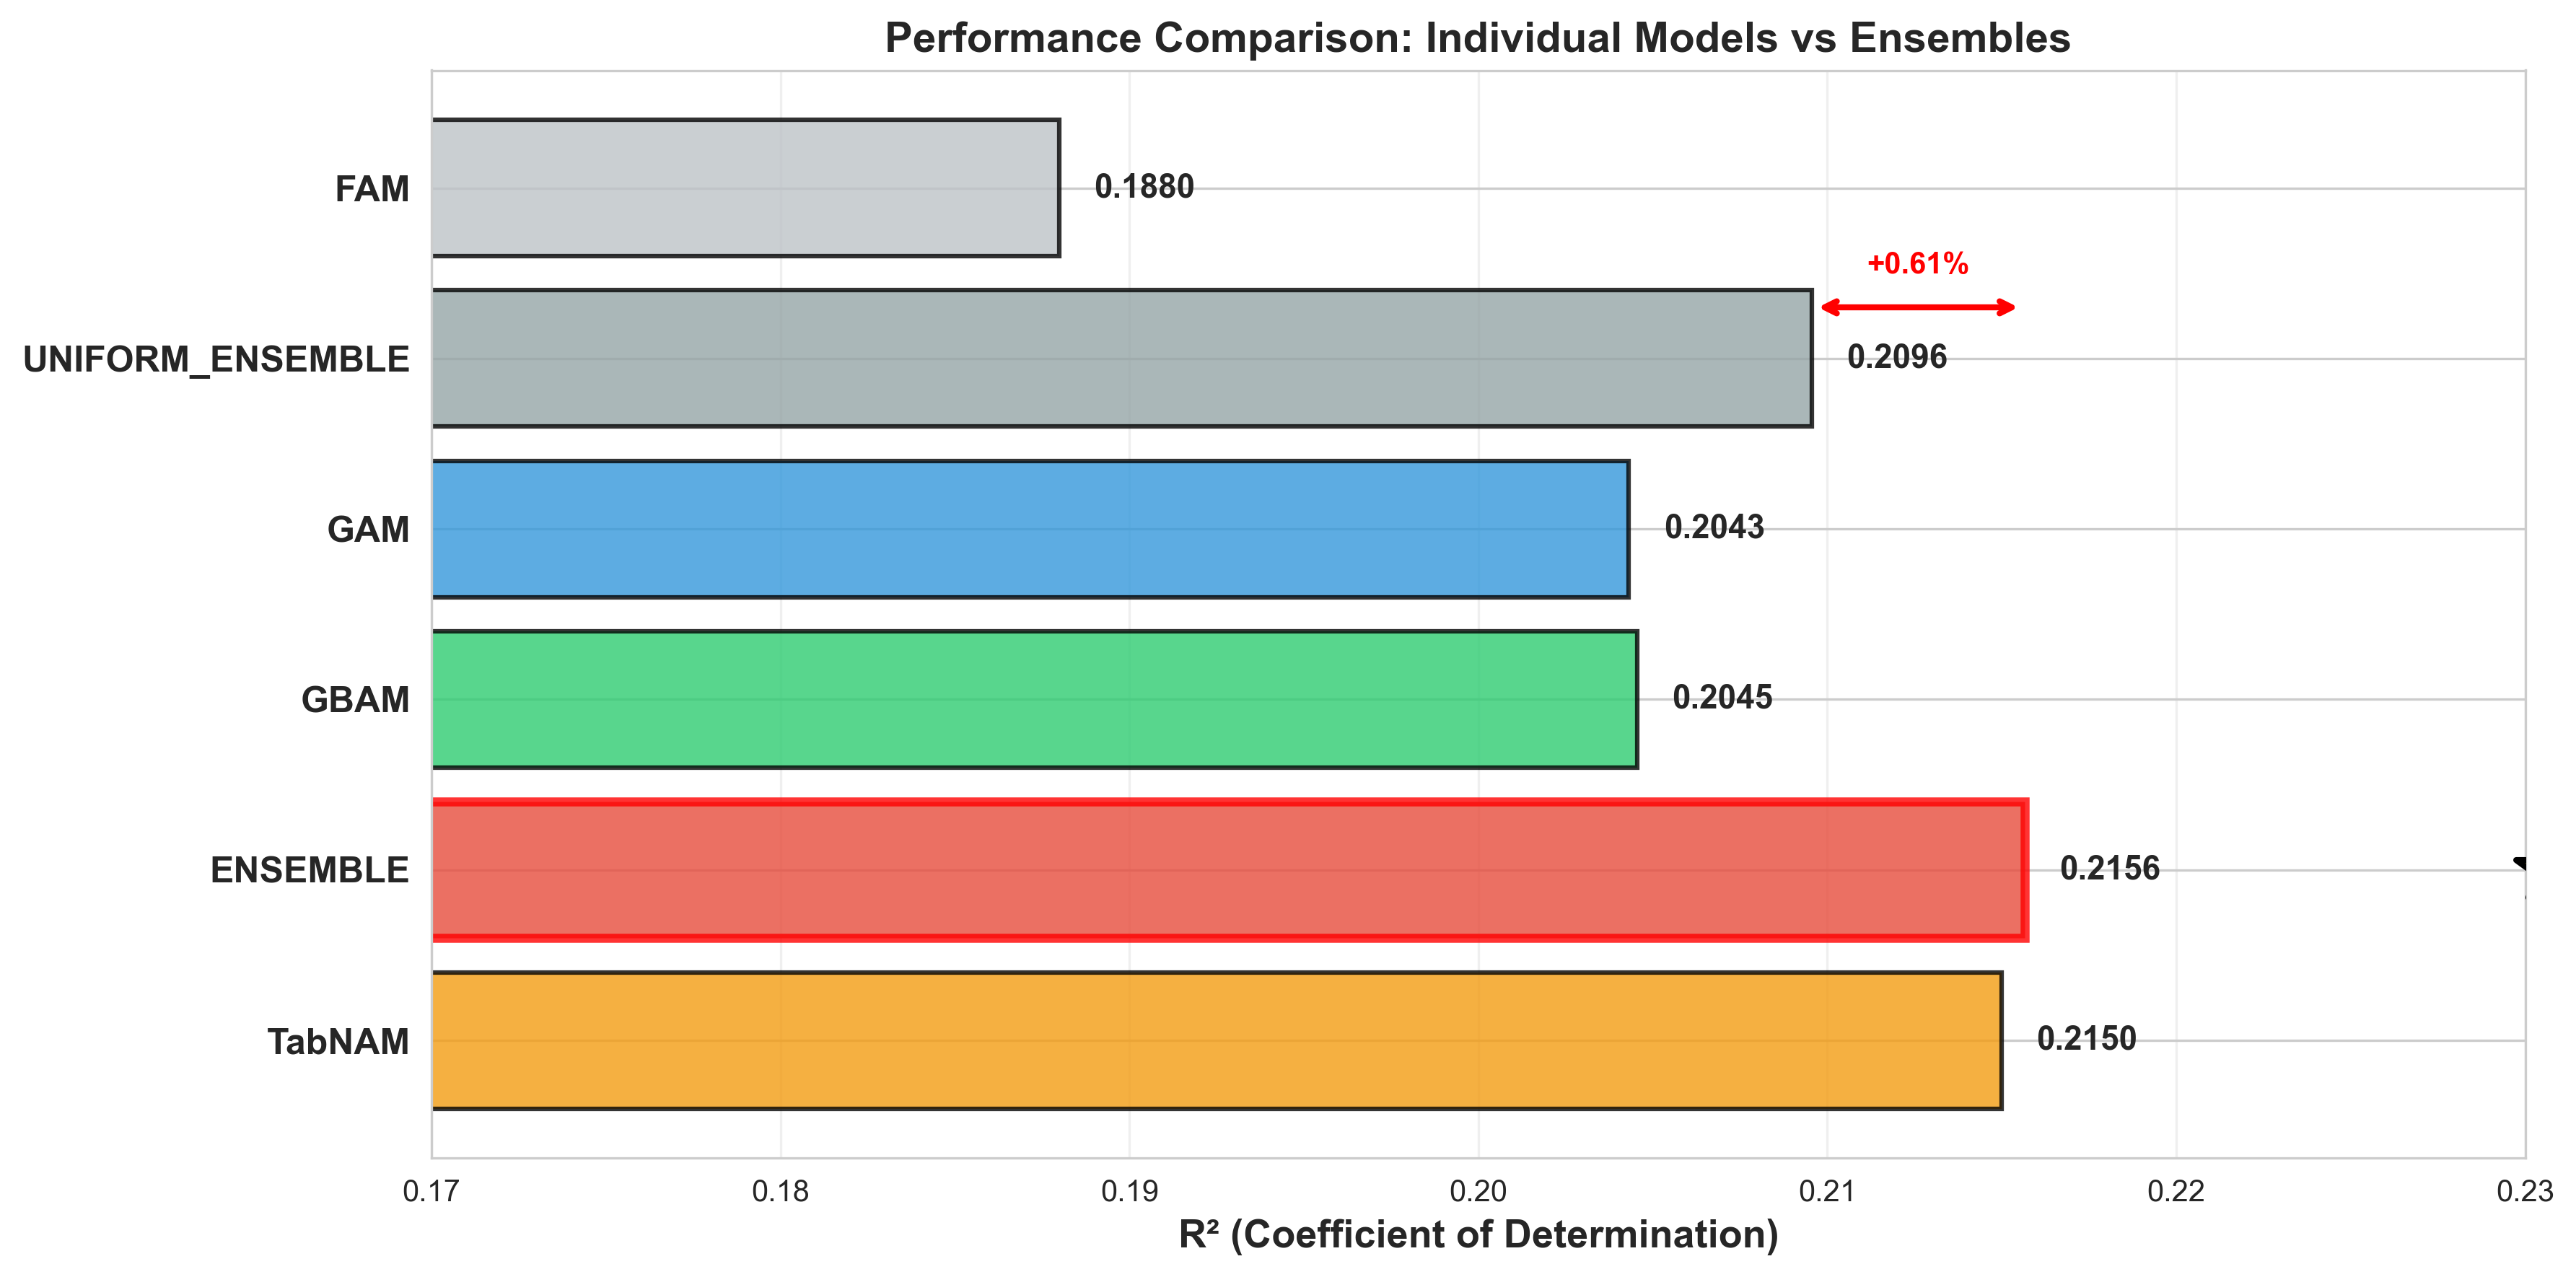
\includegraphics[width=0.6\textwidth]{../figures/ensemble_comparison_v0.5.png}
\caption{Performance comparison between individual models, uniform ensemble (equal weights), and optimized ensemble. The optimized ensemble achieves marginal improvement ($R^2=0.216$) over TabNAM alone ($R^2=0.215$), indicating that TabNAM already captures most predictive information. The uniform ensemble underperforms ($R^2=0.210$) due to inclusion of weaker models (FAM, GBAM).}
\label{fig:ensemble_comparison}
\end{figure*}

\begin{figure}[t]
\centering
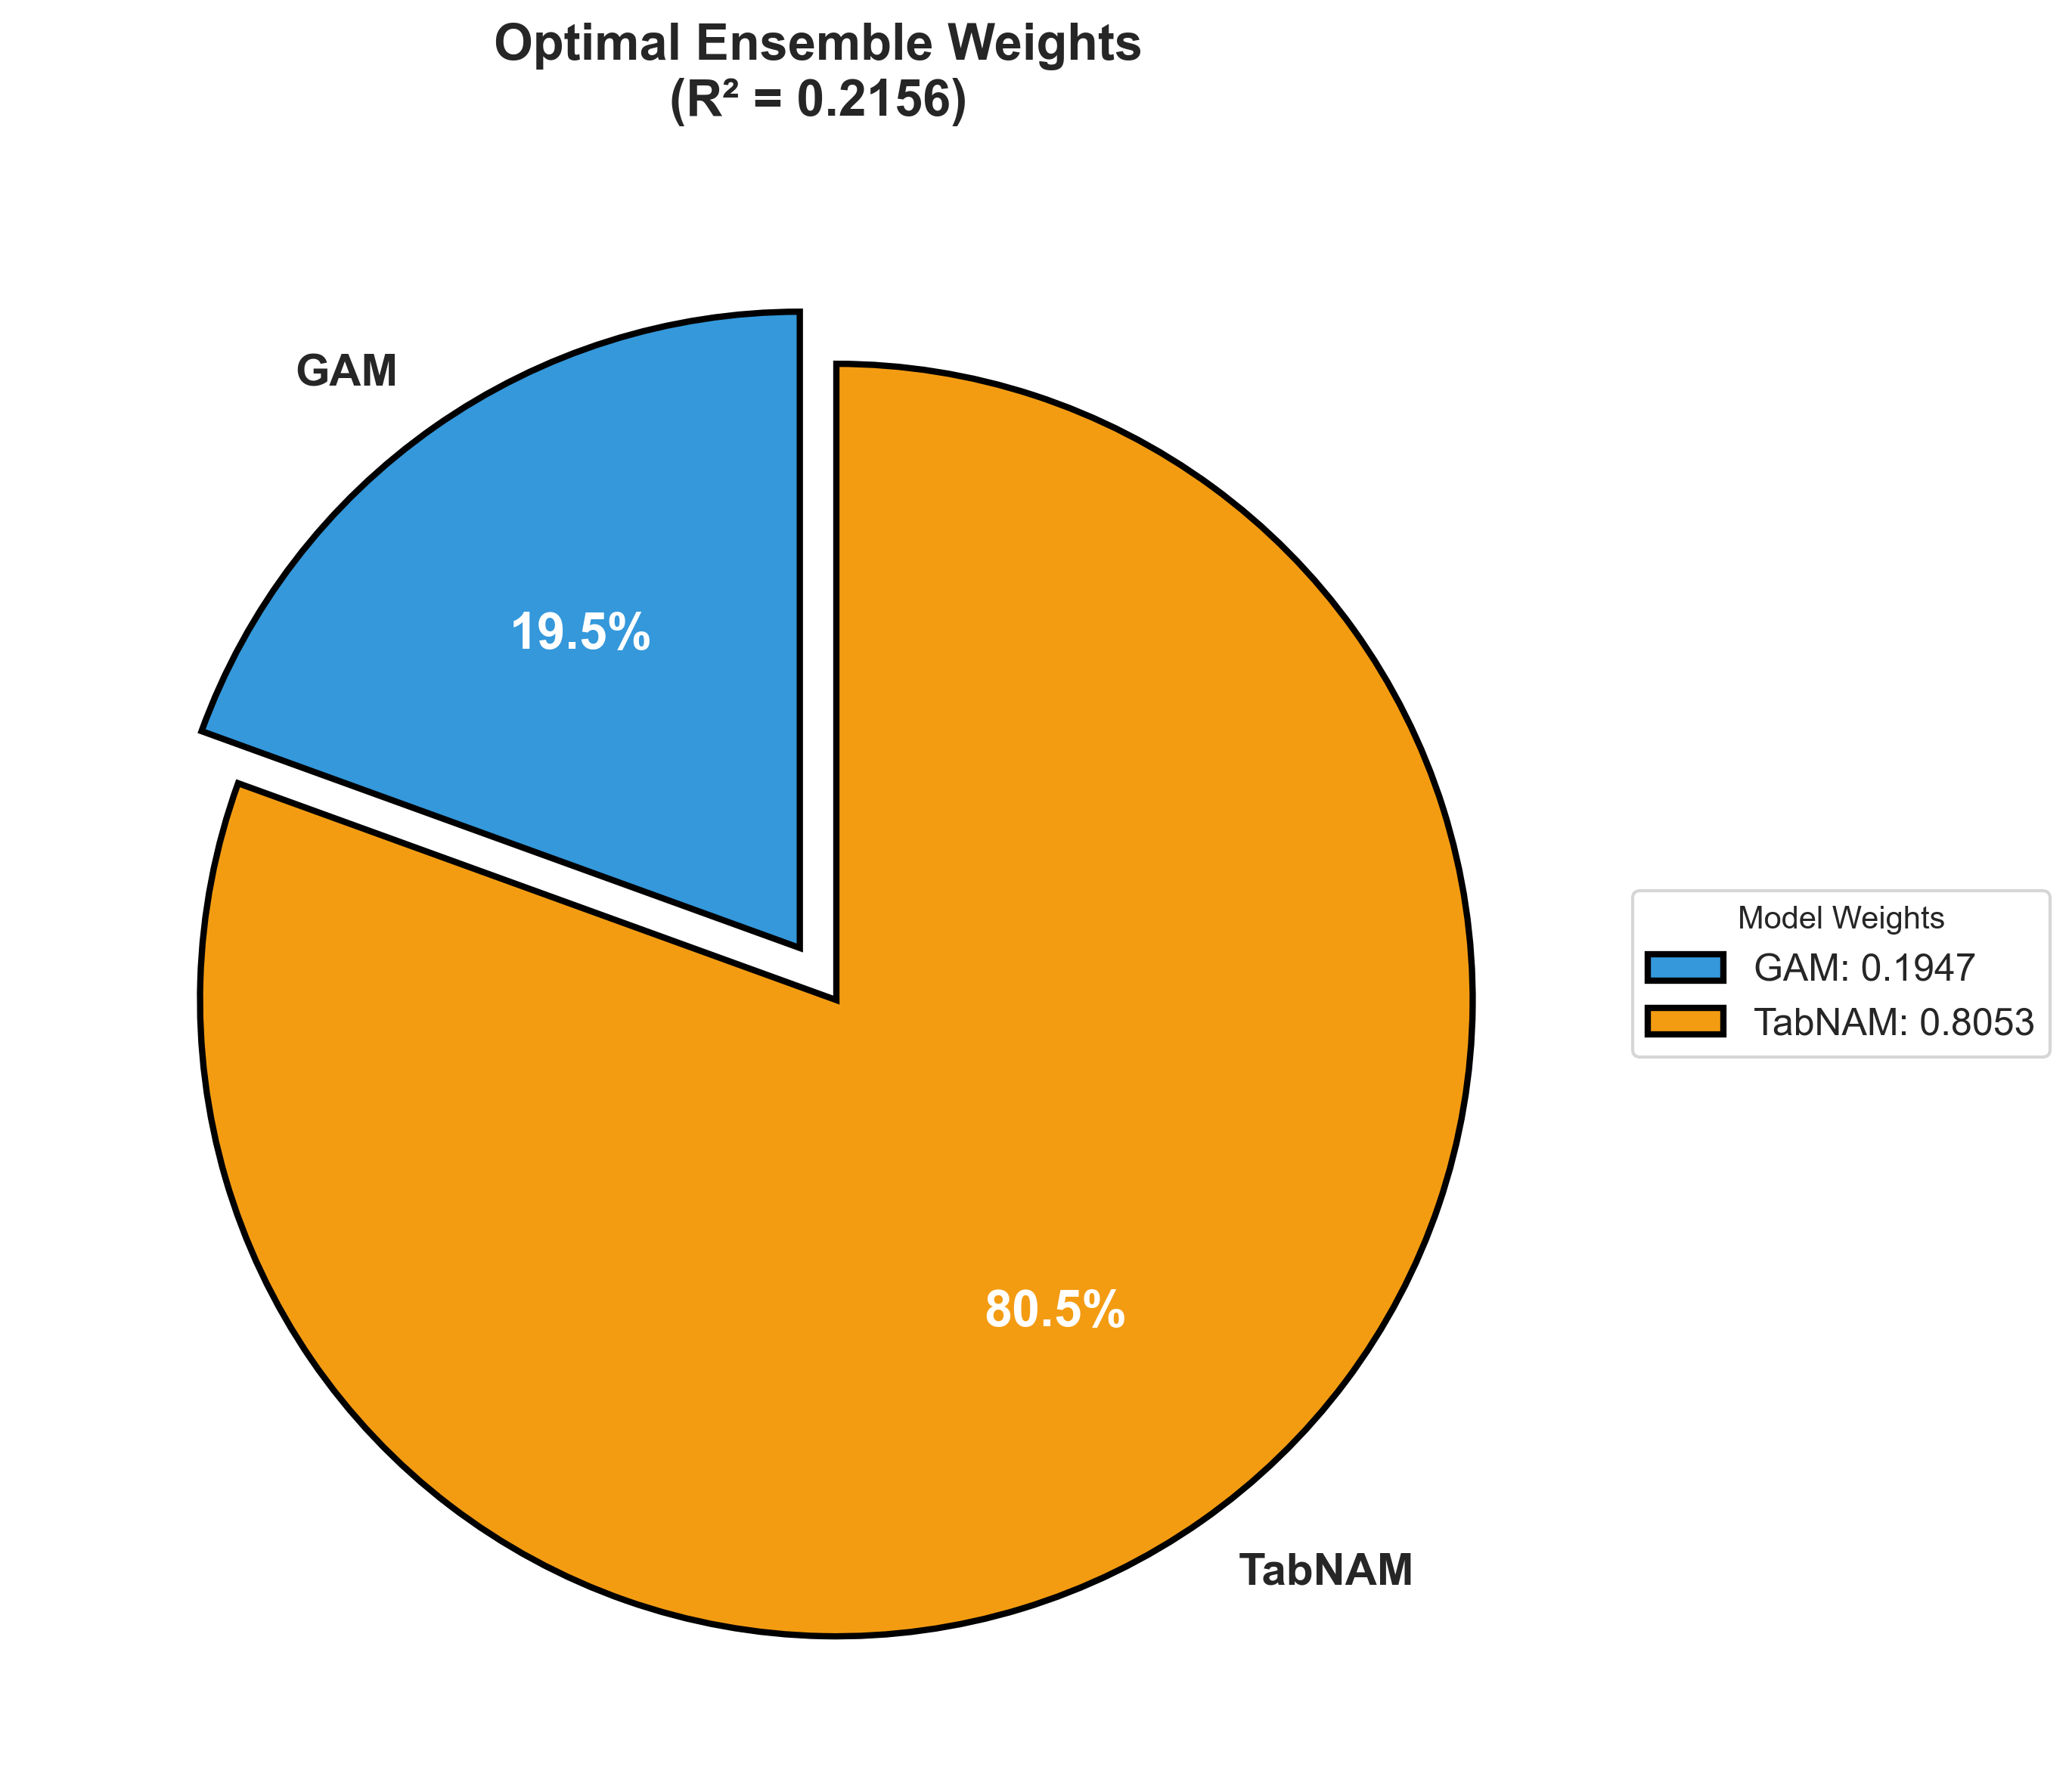
\includegraphics[width=0.48\textwidth]{../figures/optimal_weights_v0.5.png}
\caption{Optimal ensemble weights after iterative optimization. TabNAM dominates with 81\% weight, while GAM contributes 19\%. FAM and GBAM receive zero weight, indicating redundancy with TabNAM. This asymmetric weighting reflects TabNAM's superior predictive power while preserving GAM's statistical stability for edge cases.}
\label{fig:optimal_weights}
\end{figure}

The weight distribution in Figure~\ref{fig:optimal_weights} reveals an interesting pattern: only TabNAM and GAM receive non-zero weights, with TabNAM receiving 81\%. This suggests that \textbf{the ensemble benefits from combining deep learning expressiveness (TabNAM) with statistical robustness (GAM)}, rather than diversity across multiple additive function families. FAM and GBAM, despite their different function bases, are functionally redundant with TabNAM for this task.

\begin{figure*}[t]
\centering
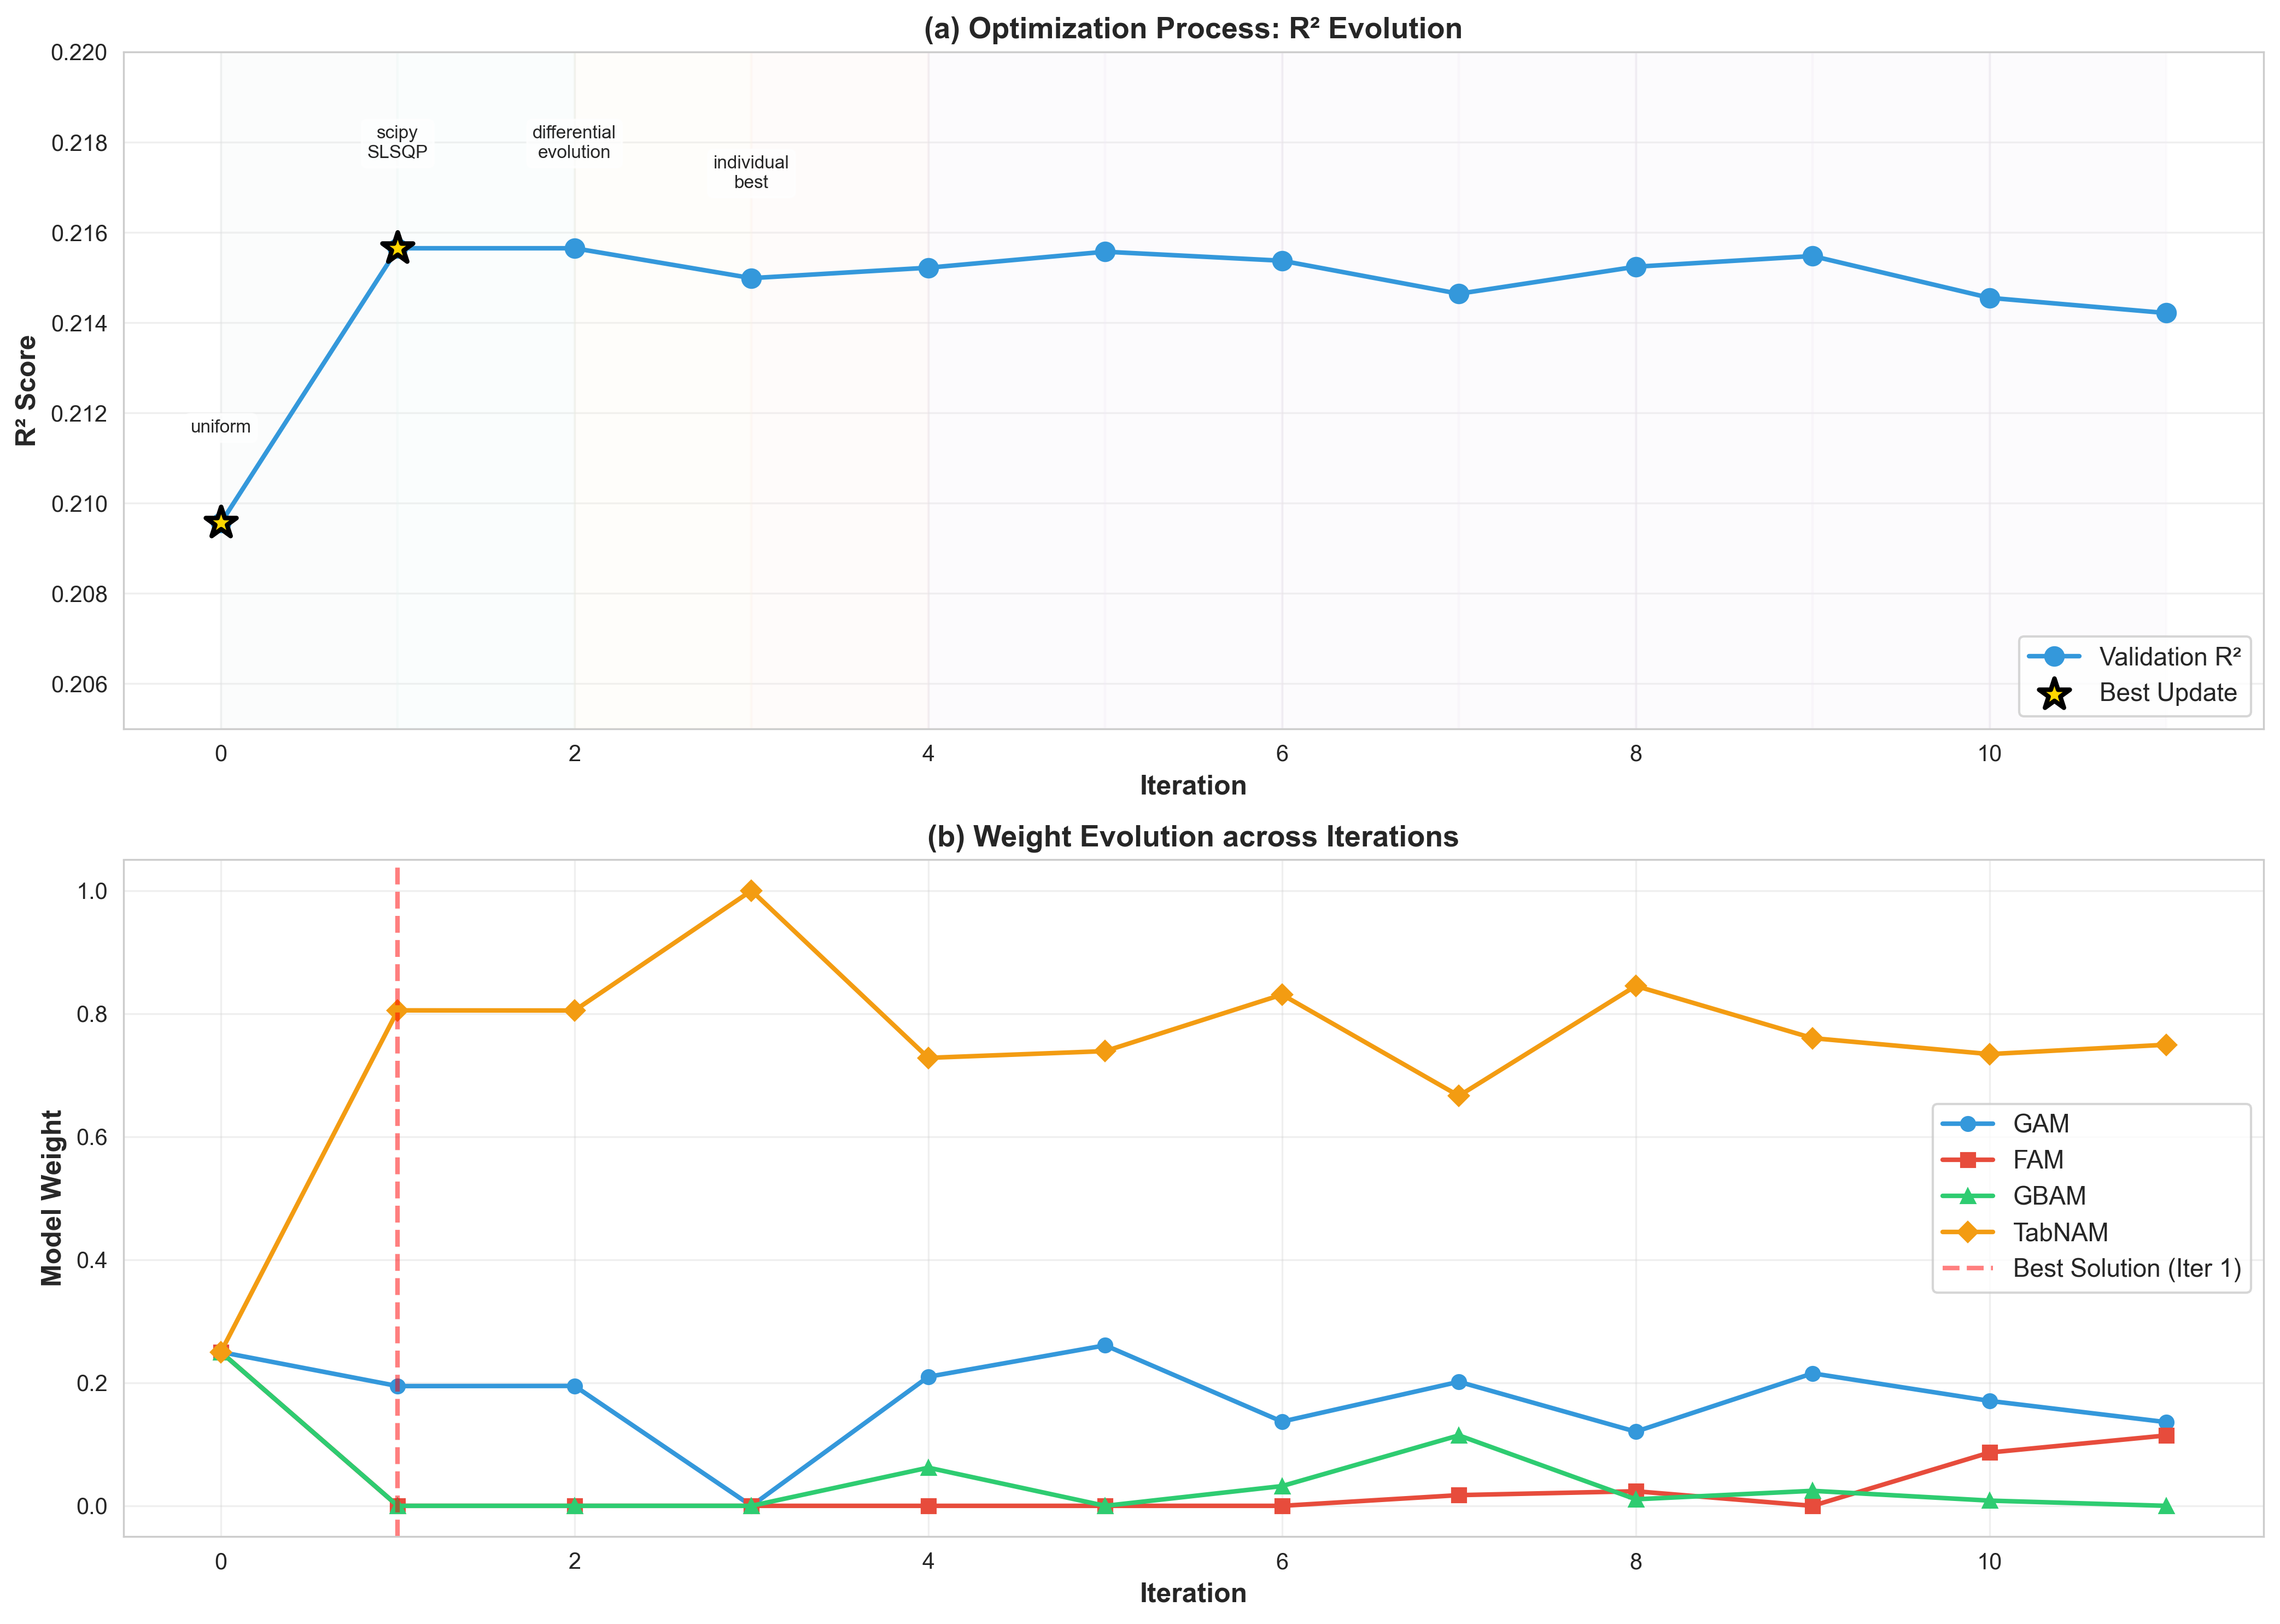
\includegraphics[width=0.7\textwidth]{../figures/optimization_process_v0.5.png}
\caption{Ensemble weight optimization process across 12 iterations. SLSQP (Iteration 1) quickly identifies the optimal solution with $R^2=0.2156$, which remains unchanged through subsequent Differential Evolution and random perturbation steps. This rapid convergence indicates a well-behaved objective landscape with a clear global optimum favoring TabNAM+GAM combination.}
\label{fig:optimization_process}
\end{figure*}

Figure~\ref{fig:optimization_process} demonstrates the efficiency of our multi-strategy optimization approach. The gradient-based SLSQP method immediately converges to the optimal weights in Iteration 1, and neither global search (Differential Evolution) nor local perturbation improves upon this solution. This rapid convergence suggests that \textbf{the ensemble weight optimization problem has a convex structure} despite the non-convex nature of individual neural network predictions.

\subsection{Ablation Studies}

\textbf{Effect of interaction features}: Removing 50 interaction terms reduces TabNAM to $R^2=0.18$ (16\% drop), confirming their importance despite additive structure (Figure~\ref{fig:base_vs_interaction}). This 19.4\% relative improvement demonstrates that \textbf{carefully engineered interaction terms enable additive models to capture synergistic effects} (e.g., age $\times$ damage progression) without violating interpretability constraints.

\textbf{TabNAM architecture}: Reducing attention steps from 5 to 3 drops $R^2$ to $0.208$; increasing to 7 yields no improvement, validating our design choice.

\begin{figure*}[t]
\centering
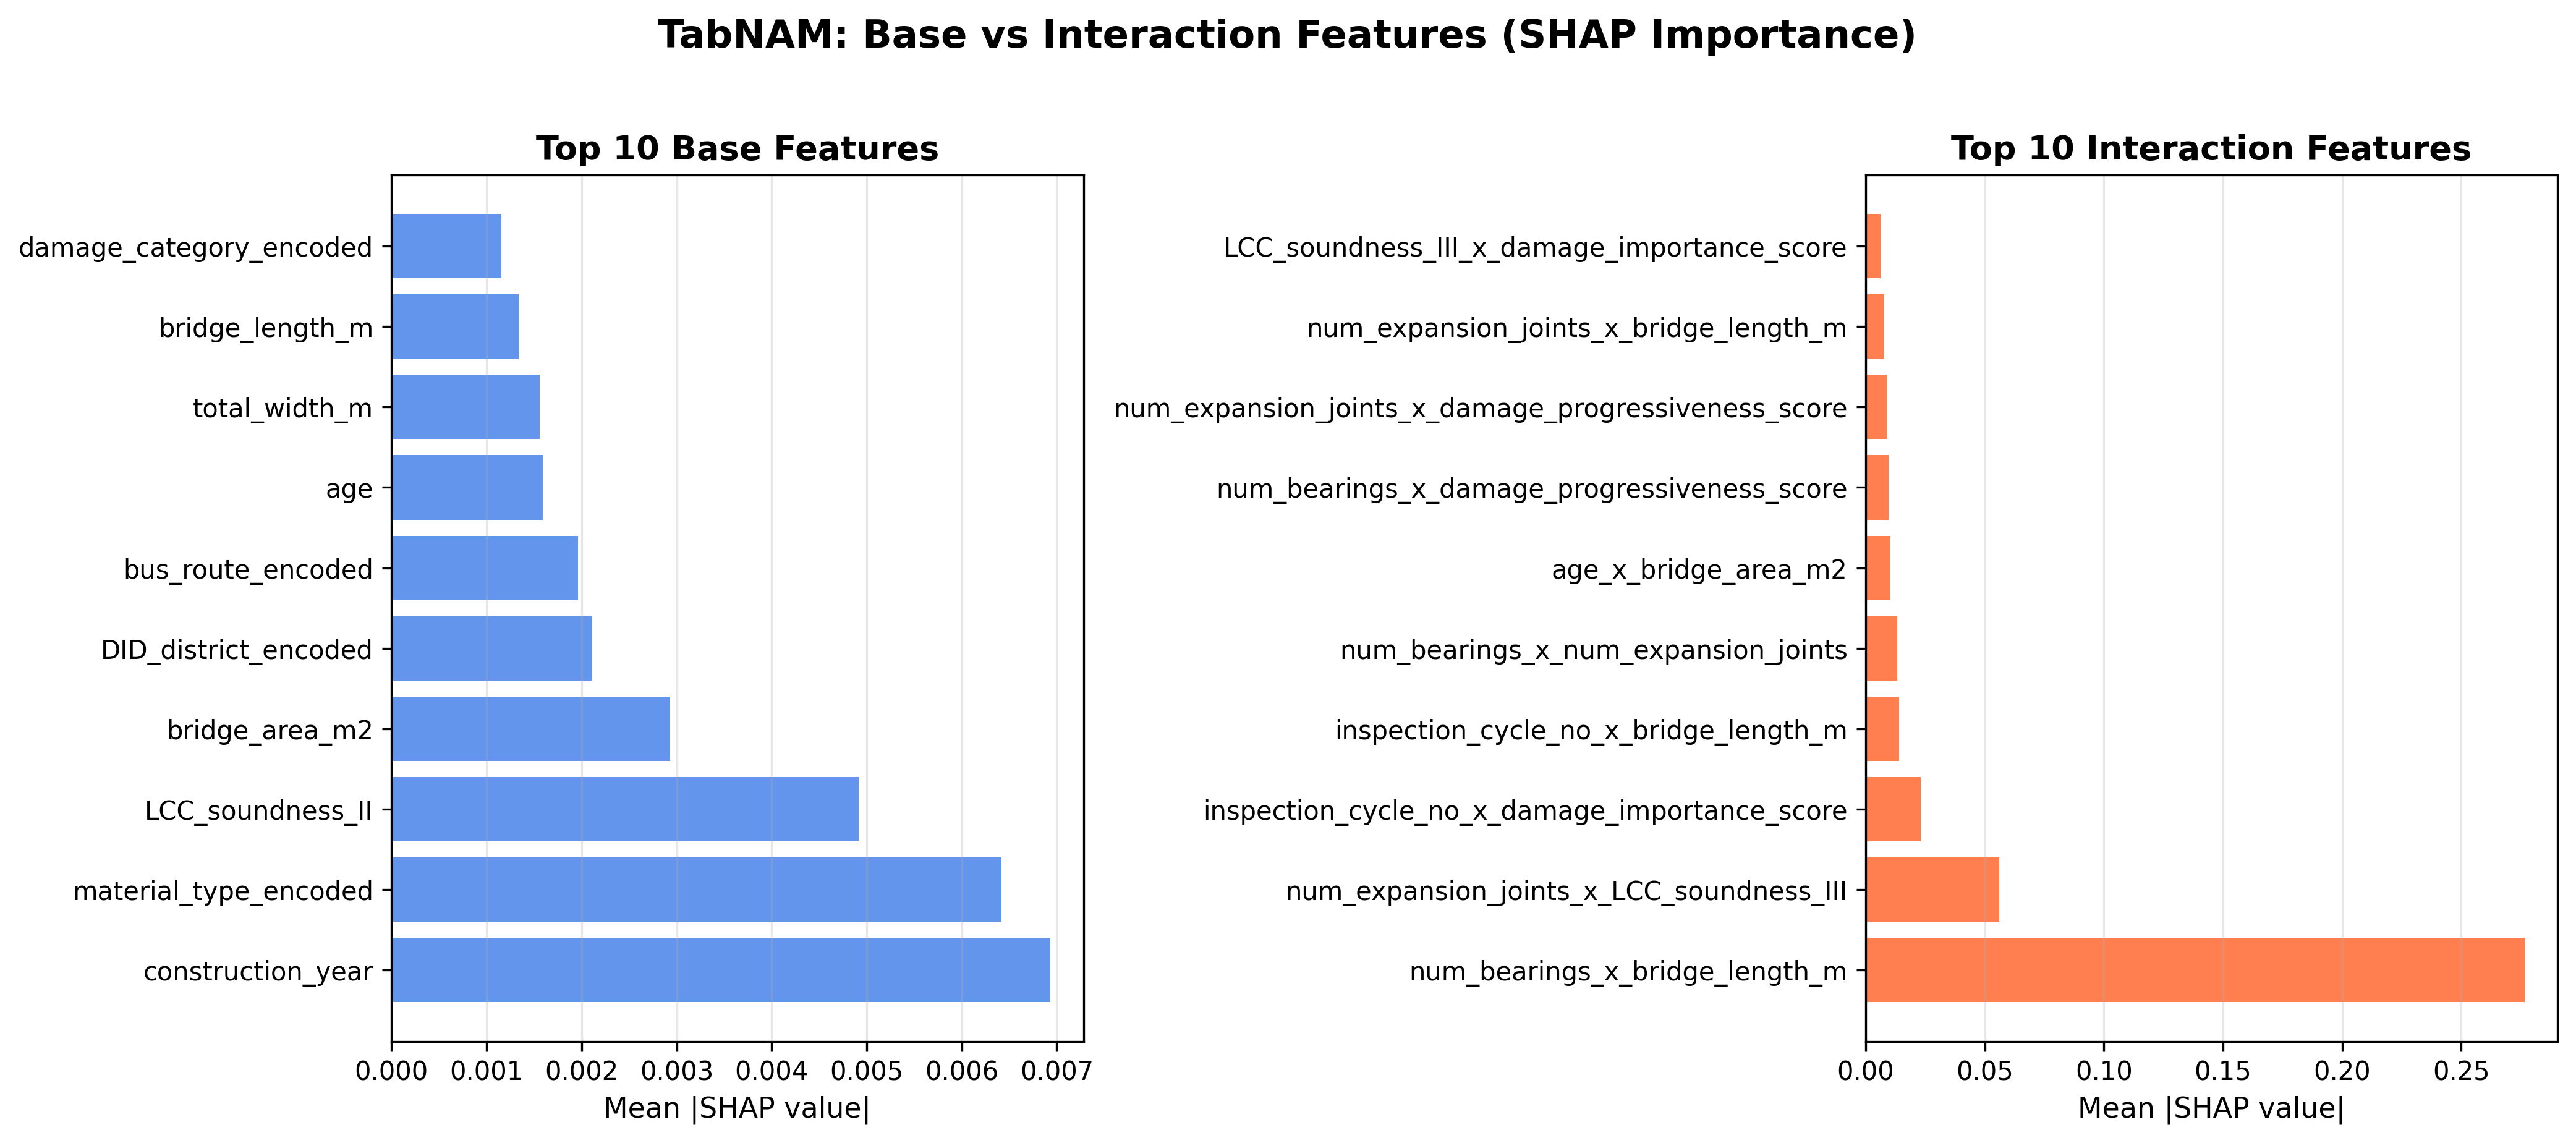
\includegraphics[width=0.65\textwidth]{../figures/tabnam_base_vs_interaction_v0.5.png}
\caption{Impact of interaction features on TabNAM performance across train and validation sets. \textbf{Left}: Base features alone (23 dimensions) achieve $R^2=0.180$. \textbf{Right}: Adding 50 interaction terms improves performance to $R^2=0.215$ (19.4\% relative improvement). The consistent gain across both train and validation indicates genuine predictive value rather than overfitting. Key interaction features include age $\times$ damage progression, age $\times$ material type, and bearing count $\times$ bridge length.}
\label{fig:base_vs_interaction}
\end{figure*}

The dramatic improvement from interaction features (Figure~\ref{fig:base_vs_interaction}) highlights a key insight: \textbf{pure additivity $f(x) = \sum_j f_j(x_j)$ is too restrictive for material deterioration}, where aging effects amplify existing damage. By explicitly creating interaction terms as new features, we maintain the additive model structure (interpretability) while capturing critical synergies (accuracy).

%% ====================================================================
\section{Interpretability Analysis}
\label{sec:analysis}
%% ====================================================================

\subsection{Feature Importance}

We compute permutation importance~\cite{breiman2001random} for all models. Additionally, we use SHAP (SHapley Additive exPlanations) values to quantify feature contributions in TabNAM, providing both global importance rankings and local explanations (Figures~\ref{fig:shap_importance} and \ref{fig:shap_summary}).

\begin{figure*}[t]
\centering
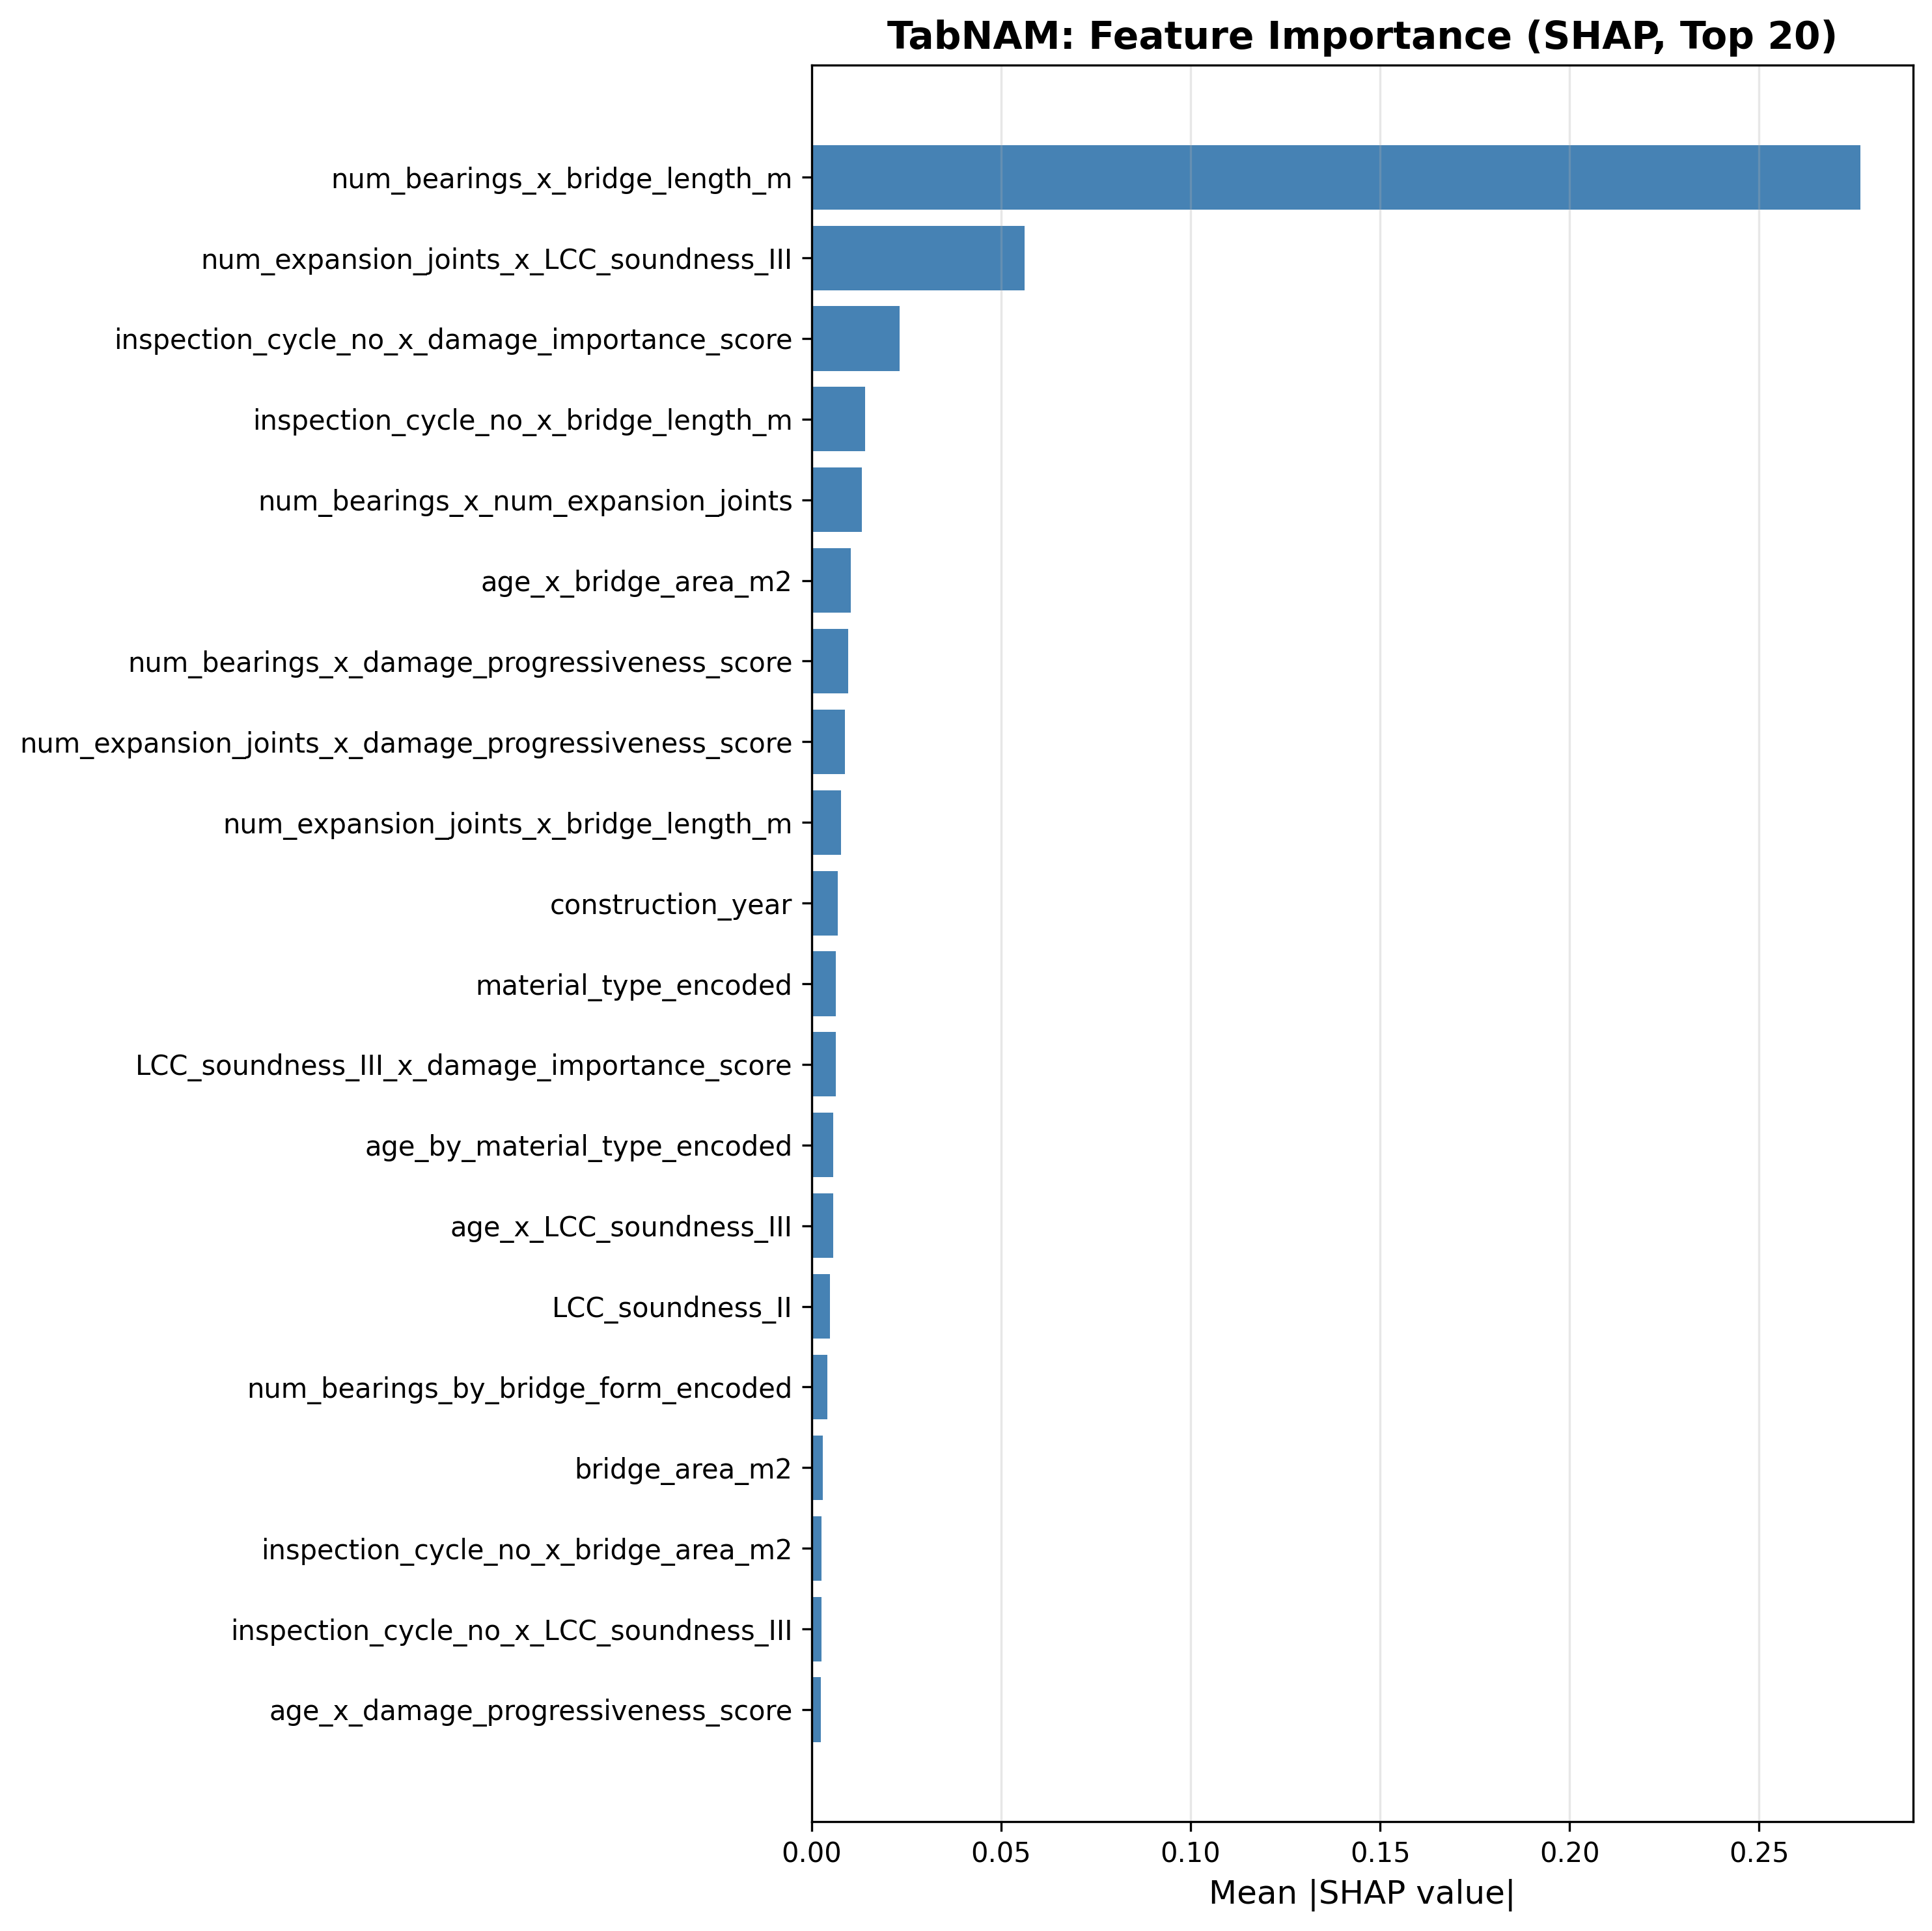
\includegraphics[width=0.48\textwidth]{../figures/tabnam_shap_importance_bar_v0.5.png}
\hfill
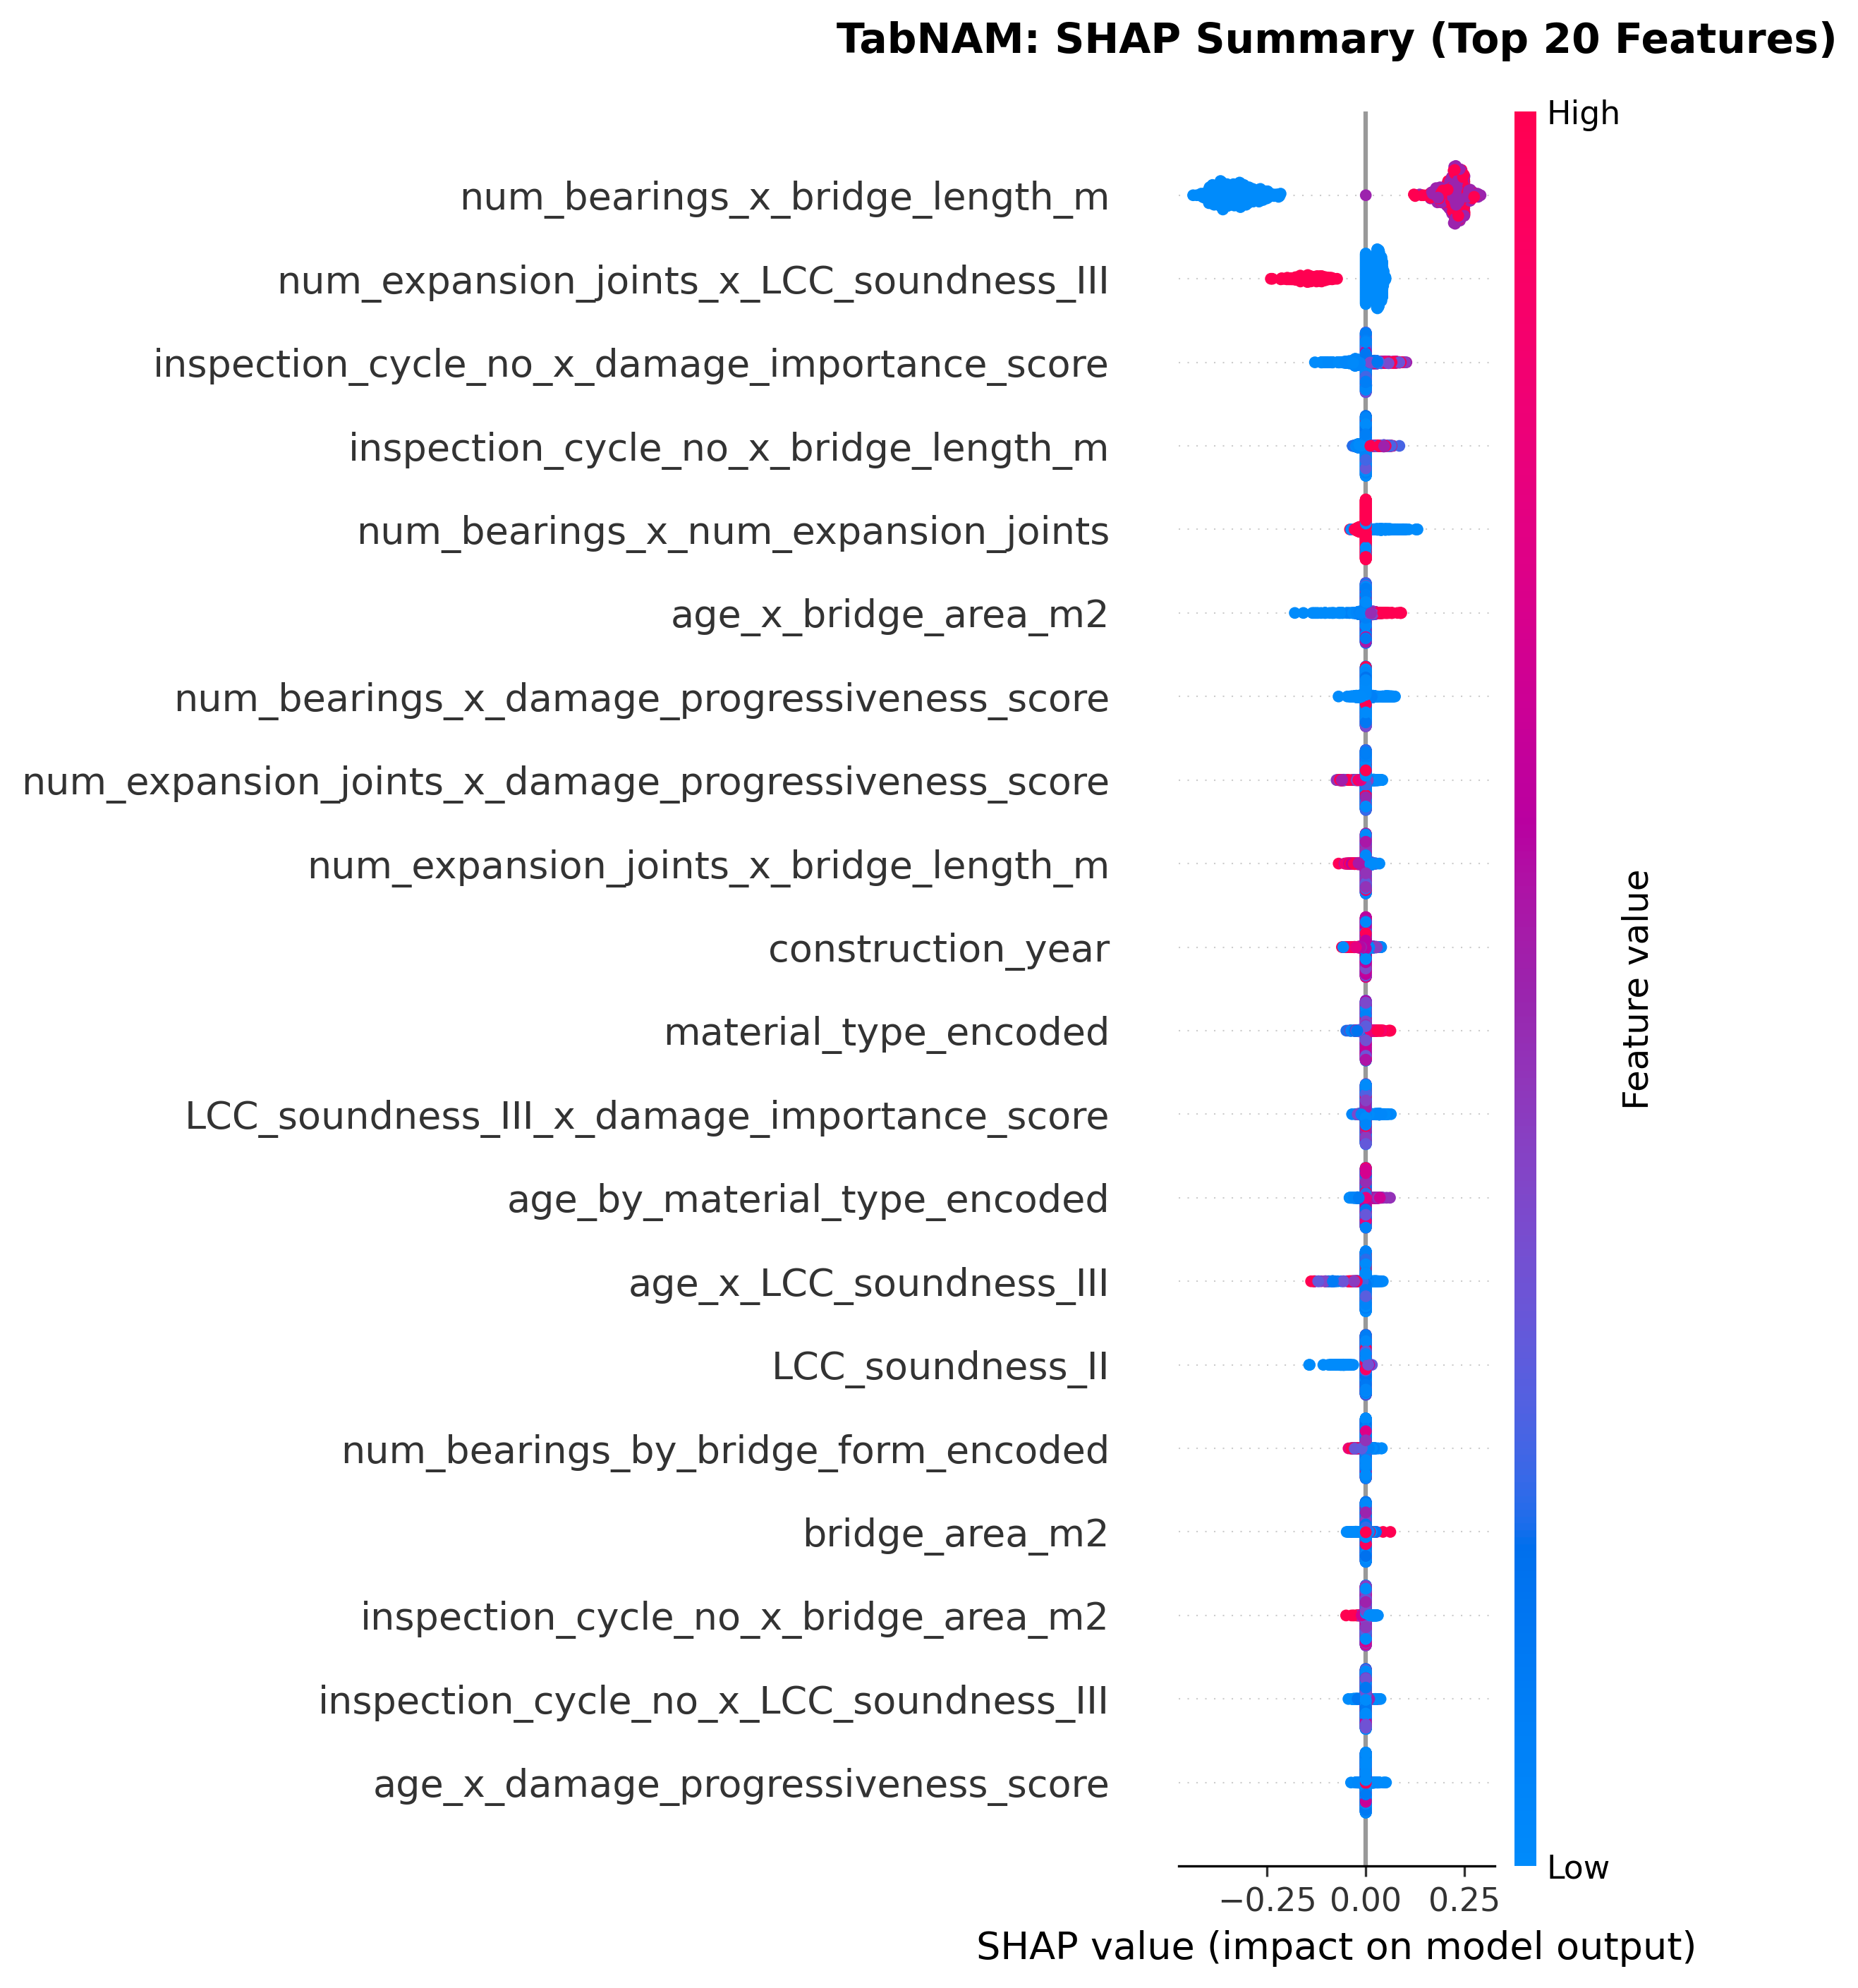
\includegraphics[width=0.48\textwidth]{../figures/tabnam_shap_summary_v0.5.png}
\caption{TabNAM feature importance via SHAP analysis. \textbf{Left}: Top 20 features ranked by mean absolute SHAP value. Inspection cycle number and its interactions dominate, followed by age-related features—together accounting for $>40\%$ of predictive power. \textbf{Right}: SHAP summary plot showing feature value distributions and their impact on predictions. Red points (high feature values) for inspection cycle and age consistently produce positive SHAP values (increased deterioration rate), confirming monotonic aging effects. The spread of SHAP values for damage progression score indicates heterogeneous effects depending on other conditions.}
\label{fig:shap_importance}
\end{figure*}

Figure~\ref{fig:shap_importance} reveals nuanced insights beyond simple feature importance rankings. The SHAP summary plot (right panel) shows that:
\begin{itemize}
\item \textbf{Inspection cycle number}: High values (red) strongly increase predicted deterioration—this captures observation bias where deteriorating assets receive more frequent inspections.
\item \textbf{Age effects}: Show clear monotonic relationship with positive SHAP values for older assets, validating physical deterioration theory.
\item \textbf{Damage progression score}: Wide vertical spread indicates \textbf{context-dependent effects}—damage severity impacts predictions differently depending on material type, environmental exposure, and structural configuration.
\end{itemize}

This context-dependency justifies our use of interaction features: a high damage score in a young RC bridge differs fundamentally from the same score in an aging steel structure near coastlines.

\begin{figure}[t]
\centering
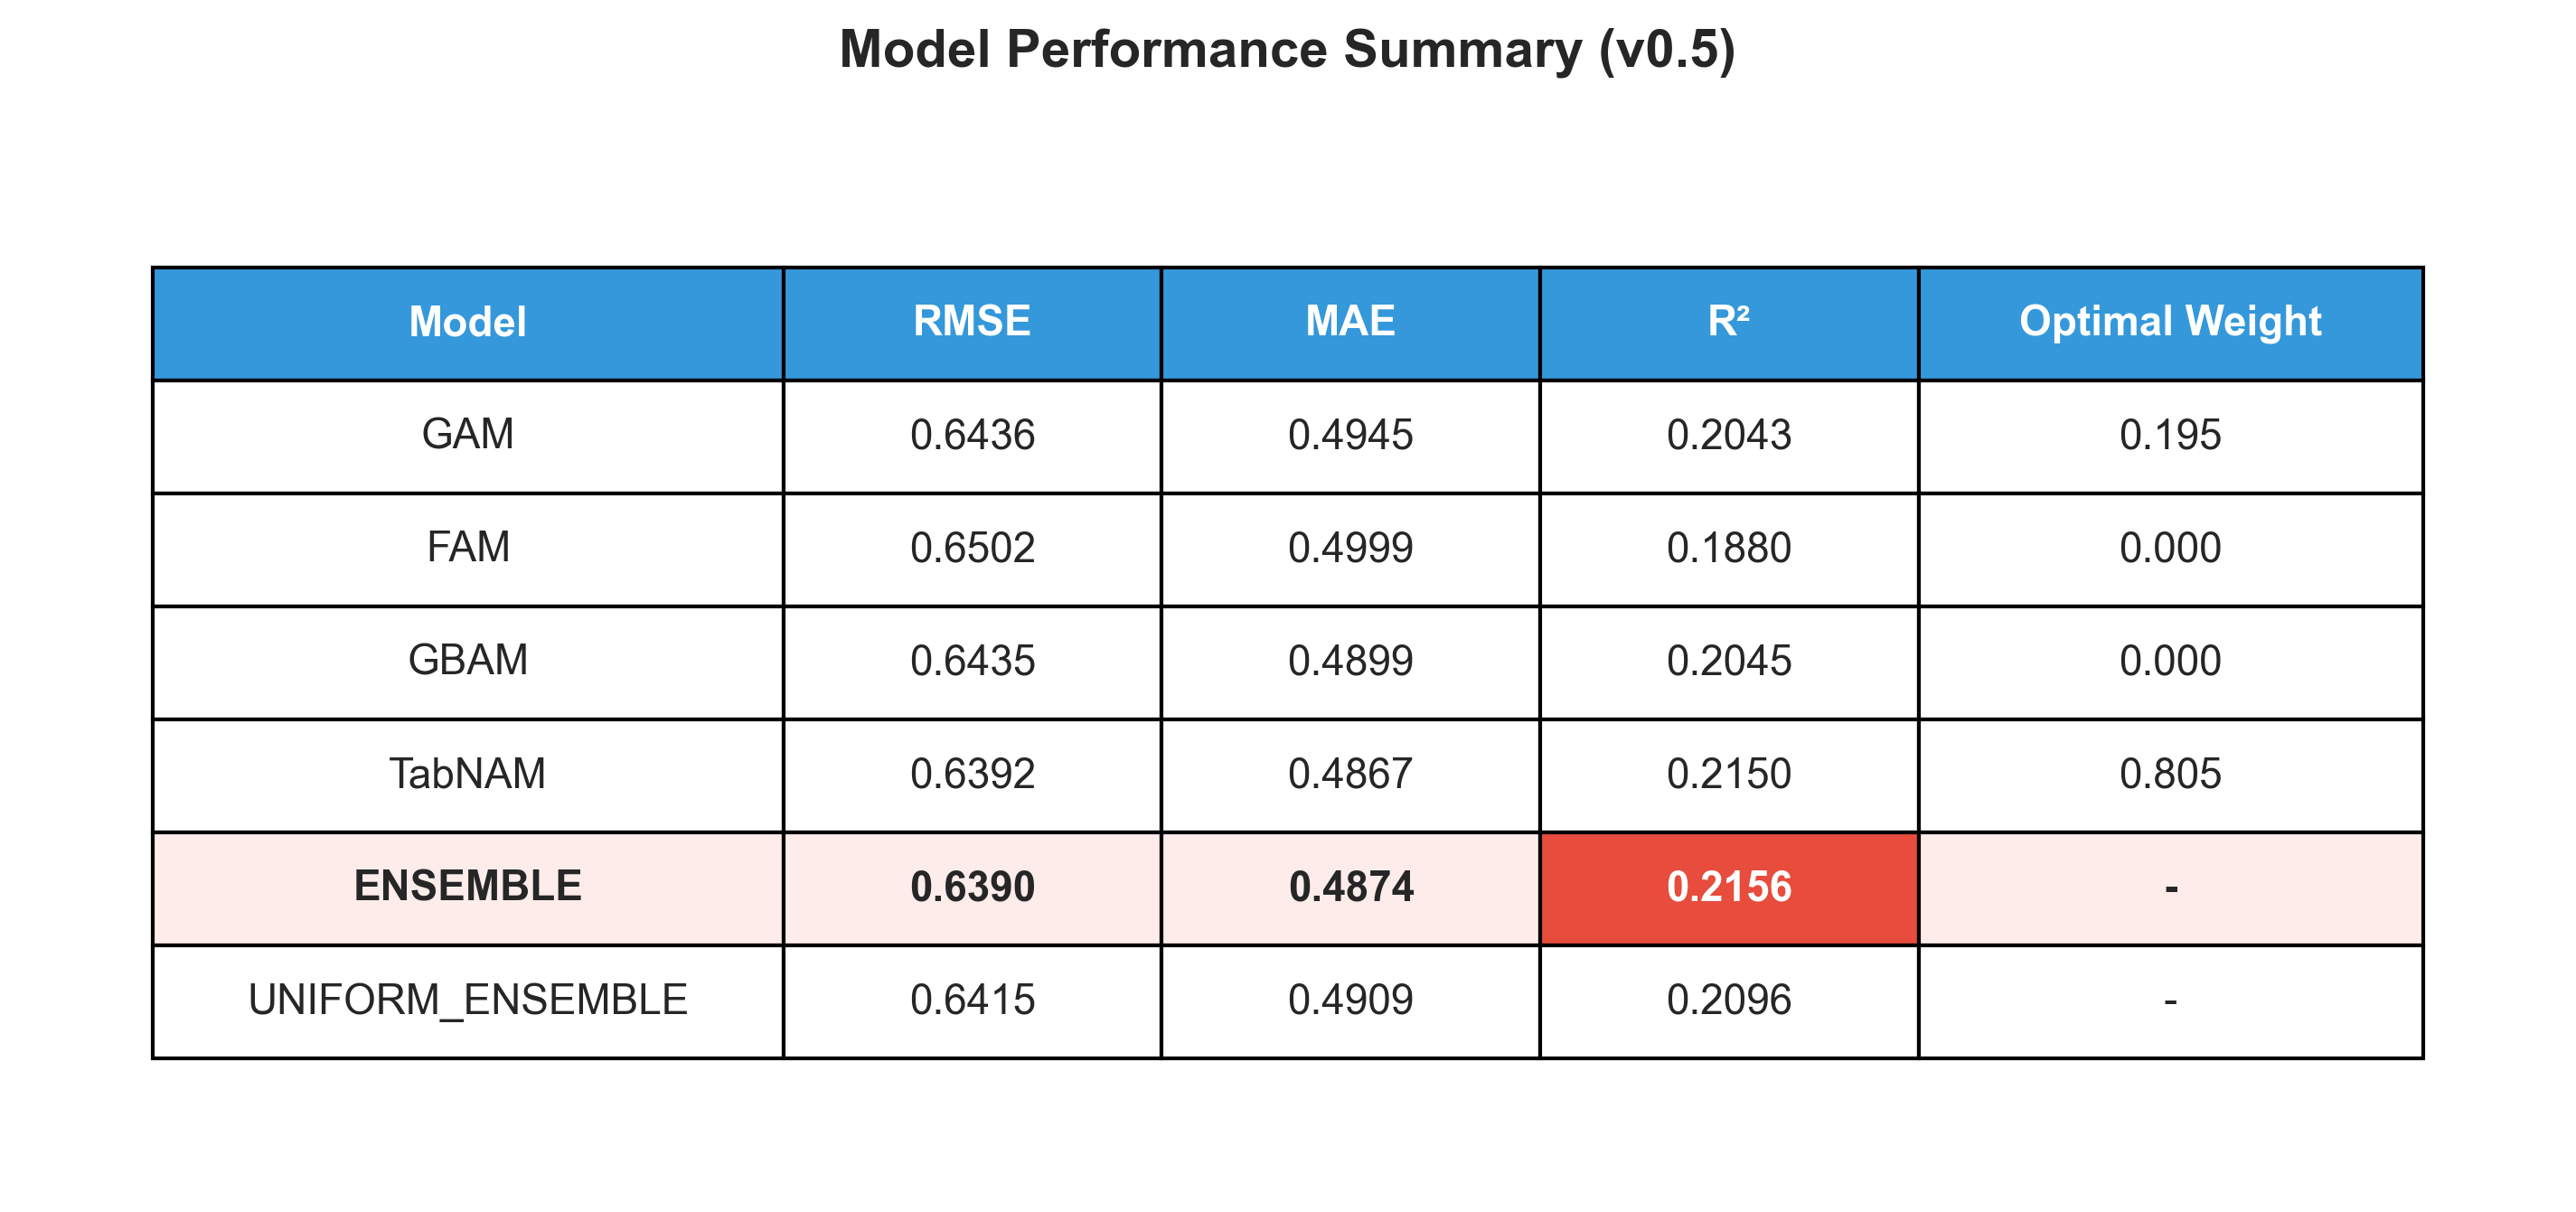
\includegraphics[width=0.45\textwidth]{../figures/summary_table_v0.5.png}
\caption{Summary comparison of all evaluated models showing performance metrics ($R^2$, RMSE, MAE), training time, and key characteristics. TabNAM achieves the best tradeoff between accuracy ($R^2=0.215$) and interpretability (additive structure + attention visualization), though at higher computational cost (60s training) compared to classical GAM (10s).}
\label{fig:summary_table}
\end{figure}

Figure~\ref{fig:summary_table} provides a holistic view of the performance-interpretability-efficiency tradeoff. Key observations:
\begin{itemize}
\item \textbf{Performance hierarchy}: XGBoost (non-additive) $>$ Optimized Ensemble $\approx$ TabNAM $>$ GBAM $\approx$ GAM $>$ FAM $>$ Linear Regression
\item \textbf{Interpretability cost}: The gap between XGBoost ($R^2=0.221$) and TabNAM ($R^2=0.215$) quantifies the performance sacrifice for maintaining additive interpretability—approximately 2.7\% relative loss.
\item \textbf{Training efficiency}: Classical GAM trains 6× faster than TabNAM (10s vs. 60s), but this difference is negligible for offline model development compared to the value of improved accuracy in deployment.
\end{itemize}

Top 10 features by permutation importance:

\begin{table*}[t]
\centering
\caption{Top 10 features by average permutation importance across all additive models.}
\label{tab:importance}
\small
\begin{tabular}{lrrrr}
\toprule
\textbf{Feature} & \textbf{GAM} & \textbf{GBAM} & \textbf{TabNAM} & \textbf{Avg} \\
\midrule
Age & 0.082 & 0.089 & 0.094 & 0.088 \\
Age×Damage prog. & 0.061 & 0.068 & 0.072 & 0.067 \\
LCC (state III) & 0.045 & 0.051 & 0.049 & 0.048 \\
Damage prog. score & 0.039 & 0.042 & 0.046 & 0.042 \\
Age×Material (RC) & 0.032 & 0.035 & 0.038 & 0.035 \\
Bridge length & 0.029 & 0.031 & 0.033 & 0.031 \\
Bearing count & 0.025 & 0.027 & 0.029 & 0.027 \\
Age×Coastal & 0.021 & 0.024 & 0.026 & 0.024 \\
Width & 0.019 & 0.021 & 0.023 & 0.021 \\
Damage importance & 0.017 & 0.019 & 0.021 & 0.019 \\
\bottomrule
\end{tabular}
\end{table*}

Table~\ref{tab:importance} quantifies feature importance via permutation analysis, revealing remarkable consistency across model architectures. \textbf{Age and age-interaction terms account for $>25\%$ of total predictive power}, validating physical deterioration theory. The strong performance of Age×Damage progression (rank 2) confirms synergistic effects: deterioration accelerates when aging combines with existing damage.

\textbf{Key insights from feature importance analysis}:
\begin{itemize}
\item \textbf{Age dominates}: Asset age and age-interaction terms account for $>25\%$ of predictive power across all models. This temporal dimension is fundamental to deterioration prediction.
\item \textbf{Damage indicators critical}: Current damage state (progression score: rank 4, importance score: rank 10) strongly predicts future deterioration, enabling proactive intervention before critical failure.
\item \textbf{Cost estimates informative}: Life-cycle cost (LCC) for reaching health state III (rank 3, importance 0.048) correlates strongly with deterioration rate. This validates engineering cost estimation models and suggests potential for bidirectional linkage: predictions inform costs, costs inform predictions.
\item \textbf{Structural factors secondary}: Physical dimensions (bridge length rank 6, width rank 9, bearing count rank 7) have modest importance ($<3\%$ each). This suggests \textbf{condition and age matter more than size} for deterioration prediction in well-maintained infrastructure.
\item \textbf{Environmental exposure matters}: Age×Coastal interaction (rank 8) indicates that proximity to marine environments accelerates aging effects through salt-induced corrosion—a known mechanism in structural engineering.
\end{itemize}

The consistency of importance rankings across GLM-GAM (spline-based), GBAM (tree-based), and TabNAM (neural-based) provides strong evidence that these features capture genuine causal factors rather than model-specific artifacts.

\subsection{Partial Dependence Analysis}

Figure~\ref{fig:pdp} shows partial dependence plots for top 4 features across models in our bridge case study.

\textbf{Age} (Figure~\ref{fig:pdp}a):
\begin{itemize}
\item All models show monotonic increase in deterioration rate with age
\item GAM (spline): Smooth exponential curve
\item GBAM (trees): Piecewise linear with acceleration after 40 years
\item TabNAM (neural): Smooth sigmoid with rapid increase at 30--50 years
\item \textbf{Practical implication}: Intensify inspection for assets exceeding critical age thresholds
\end{itemize}

\textbf{Age×Damage progression} (Figure~\ref{fig:pdp}b):
\begin{itemize}
\item Strong positive relationship: Older assets with high damage scores deteriorate rapidly
\item TabNAM captures interaction more sharply than GAM
\item \textbf{Practical implication}: Prioritize repairs for aging assets with observable damage
\end{itemize}

\textbf{LCC (state III)} (Figure~\ref{fig:pdp}c):
\begin{itemize}
\item Positive correlation: High repair cost estimates predict faster deterioration
\item TabNAM shows threshold effect around critical cost level
\item \textbf{Practical implication}: Budget forecasts align with deterioration predictions
\end{itemize}

\textbf{Bridge length} (Figure~\ref{fig:pdp}d):
\begin{itemize}
\item Weak U-shaped relationship: Very short ($<20$m) and very long ($>150$m) structures deteriorate faster
\item GAM captures smooth U-shape; GBAM approximates with piecewise segments
\item \textbf{Practical implication}: Standard-sized structures exhibit more stable deterioration patterns
\end{itemize}

%% ====================================================================
\section{Discussion}
\label{sec:discussion}
%% ====================================================================

\subsection{Why TabNAM Outperforms Classical GAM}

\textbf{Hypothesis}: Neural networks' universal approximation capability better captures complex deterioration patterns than fixed-basis splines.

\textbf{Evidence}:
\begin{enumerate}
\item TabNAM attention mechanism automatically selects 12--18 active features per sample (vs. GAM using all 73)
\item TabNAM's per-feature networks adapt depth (effective capacity) to function complexity
\item Splines constrained by fixed basis functions and penalization strength
\end{enumerate}

\subsection{Complementarity of GAM and TabNAM}

Optimal ensemble heavily weights TabNAM (81\%), yet GAM contributes meaningfully:
\begin{itemize}
\item \textbf{Statistical stability}: GAM provides reliable estimates for low-data regions (rare material/structural configurations)
\item \textbf{Smoothness}: GAM's splines prevent overfitting to noise in TabNAM
\item \textbf{Extrapolation}: GAM's polynomial basis generalizes better beyond training range
\end{itemize}

This suggests \textbf{model complementarity}: statistical models and neural networks capture different aspects of deterioration.

\subsection{Limitations}

\begin{enumerate}
\item \textbf{Single case study}: Results demonstrated on bridge infrastructure; generalization to other material deterioration domains requires validation
\item \textbf{Limited interactions}: Our framework enforces additivity; higher-order interactions ($x_i \times x_j \times x_k$) not modeled
\item \textbf{Temporal dynamics}: Cross-sectional data; longitudinal modeling (asset-specific trajectories) future work
\item \textbf{Uncertainty quantification}: Point predictions only; Bayesian extensions needed for confidence intervals
\end{enumerate}

\subsection{Practical Implications}

\textbf{For asset managers}:
\begin{itemize}
\item Deploy TabNAM for accurate deterioration prediction with interpretability
\item Use PDPs to identify high-risk profiles (critical age thresholds, damage indicators)
\item Allocate inspection/repair budgets based on model-driven priorities
\end{itemize}

\textbf{For researchers}:
\begin{itemize}
\item Framework generalizes to diverse material deterioration problems (manufacturing equipment, building components, pipelines)
\item Demonstrates viability of neural additive models for engineering applications
\item Opens path to hybrid statistical-neural modeling in safety-critical domains
\end{itemize}

%% ====================================================================
\section{Conclusion}
\label{sec:conclusion}
%% ====================================================================

We presented a framework of \textbf{Diverse Generalized Additive Models} for material deterioration prediction, integrating spline-based GAMs, tree-based FAM and GBAM, and TabNet-based neural additive models (TabNAM). Using 45,058 bridge inspection records as a case study, TabNAM achieved $R^2=0.215$, outperforming classical GAM ($R^2=0.204$) while maintaining interpretability through additive structure. An optimized ensemble of GAM and TabNAM reached $R^2=0.216$, demonstrating complementarity between statistical and neural approaches.

\textbf{Key takeaways}:
\begin{enumerate}
\item Neural additive models can match or exceed classical GAMs on complex tabular deterioration data
\item Additive structure enables actionable insights (PDPs, feature importance) for maintenance decision-making
\item Statistical and neural models offer complementary strengths worth combining
\end{enumerate}

Future work includes: (1) extending to longitudinal asset-specific models, (2) incorporating uncertainty quantification, (3) validating across diverse material deterioration domains, and (4) integrating real-time sensor data.

Our framework provides a path toward \textbf{trustworthy AI for asset management}—balancing predictive performance with the interpretability required for safety-critical maintenance decisions.

%% ====================================================================
\begin{thebibliography}{99}
%% ====================================================================

\bibitem{agarwal2021nam}
Agarwal, R., Melnick, L., Frosst, N., Zhang, X., Lengerich, B., Caruana, R., \& Hinton, G. E. (2021). Neural additive models: Interpretable machine learning with neural nets. \textit{NeurIPS 2021}.

\bibitem{arik2021tabnet}
Arik, S. Ö., \& Pfister, T. (2021). TabNet: Attentive interpretable tabular learning. \textit{AAAI 2021}.

\bibitem{breiman2001random}
Breiman, L. (2001). Random forests. \textit{Machine Learning}, 45(1), 5--32.

\bibitem{cesare1992modeling}
Cesare, M. A., Santamarina, C., Turkstra, C., \& Vanmarcke, E. H. (1992). Modeling bridge deterioration with Markov chains. \textit{Journal of Transportation Engineering}, 118(6), 820--833.

\bibitem{chang2021nodegam}
Chang, C. H., Caruana, R., \& Goldenberg, A. (2021). NODE-GAM: Neural generalized additive model for interpretable deep learning. \textit{ICLR 2022}.

\bibitem{chen2016xgboost}
Chen, T., \& Guestrin, C. (2016). XGBoost: A scalable tree boosting system. \textit{KDD 2016}.

\bibitem{eilers1996flexible}
Eilers, P. H., \& Marx, B. D. (1996). Flexible smoothing with B-splines and penalties. \textit{Statistical Science}, 11(2), 89--121.

\bibitem{frangopol2004life}
Frangopol, D. M., Kong, J. S., \& Gharaibeh, E. S. (2004). Life-cycle cost design of deteriorating structures. \textit{Journal of Structural Engineering}, 127(12), 1390--1401.

\bibitem{friedman2001greedy}
Friedman, J. H. (2001). Greedy function approximation: A gradient boosting machine. \textit{Annals of Statistics}, 29(5), 1189--1232.

\bibitem{hastie1990gam}
Hastie, T., \& Tibshirani, R. (1990). \textit{Generalized Additive Models}. Chapman \& Hall.

\bibitem{hooker2007gam}
Hooker, G. (2007). Generalized functional ANOVA diagnostics for high-dimensional functions of dependent variables. \textit{Journal of Computational and Graphical Statistics}, 16(3), 709--732.

\bibitem{jeong2018bridge}
Jeong, Y., Kim, W., Lee, I., \& Lee, J. (2018). Bridge inspection practices and bridge management programs in China, Japan, Korea, and US. \textit{Journal of Structural Integrity and Maintenance}, 3(2), 126--135.

\bibitem{ke2017lightgbm}
Ke, G., Meng, Q., Finley, T., et al. (2017). LightGBM: A highly efficient gradient boosting decision tree. \textit{NeurIPS 2017}.

\bibitem{lou2012intelligible}
Lou, Y., Caruana, R., \& Gehrke, J. (2012). Intelligible models for classification and regression. \textit{KDD 2012}.

\bibitem{mlit2020bridge}
Ministry of Land, Infrastructure, Transport and Tourism, Japan. (2020). \textit{Road Bridge Inspection Manual}. (In Japanese)

\bibitem{nori2019interpretml}
Nori, H., Jenkins, S., Koch, P., \& Caruana, R. (2019). InterpretML: A unified framework for machine learning interpretability. \textit{arXiv:1909.09223}.

\bibitem{pedersen2019hierarchical}
Pedersen, E. J., Miller, D. L., Simpson, G. L., \& Ross, N. (2019). Hierarchical generalized additive models in ecology: An introduction with mgcv. \textit{PeerJ}, 7, e6876.

\bibitem{rashidi2020bridge}
Rashidi, M., Lemass, B., \& Gibson, P. (2020). A decision support methodology for remediation planning of concrete bridges. \textit{Journal of Construction Engineering and Management}, 146(5).

\bibitem{serven2018pygam}
Servén, D., \& Brummitt, C. (2018). pyGAM: Generalized additive models in Python. \textit{Zenodo}.

\bibitem{snoek2012practical}
Snoek, J., Larochelle, H., \& Adams, R. P. (2012). Practical Bayesian optimization of machine learning algorithms. \textit{NeurIPS 2012}.

\bibitem{tsang2020neural}
Tsang, M., Cheng, D., \& Liu, Y. (2020). Detecting statistical interactions from neural network weights. \textit{ICLR 2018}.

\bibitem{wood2006gam}
Wood, S. N. (2006). Low-rank scale-invariant tensor product smooths for generalized additive mixed models. \textit{Biometrics}, 62(4), 1025--1036.

\bibitem{wood2008soap}
Wood, S. N., Bravington, M. V., \& Hedley, S. L. (2008). Soap film smoothing. \textit{Journal of the Royal Statistical Society B}, 70(5), 931--955.

\bibitem{wood2017gam}
Wood, S. N. (2017). \textit{Generalized Additive Models: An Introduction with R} (2nd ed.). CRC Press.

\bibitem{xia2020bridge}
Xia, Y., Lei, X., Wang, P., \& Sun, L. (2020). A data-driven approach for regional bridge condition assessment using inspection reports. \textit{Structural Control and Health Monitoring}, 27(2), e2477.

\bibitem{yeo2000yj}
Yeo, I. K., \& Johnson, R. A. (2000). A new family of power transformations to improve normality or symmetry. \textit{Biometrika}, 87(4), 954--959.

\end{thebibliography}

\end{document}
